%MEGA MAN X.TEX
\textit{Mega Man X} originated as a spin-off game derived from the beloved classic Mega Man series, initially released for the Super Famicom/SNES consoles (later extended to PC) during the period spanning 1993 to 1995~\cite{wiki:MMX}. Set a century after the events of the primary franchise timeline, the game unfolds in a world where both humans and unique robots capable of experiencing emotions coexist. In this world, the protagonist, X, is one of these special robots and finds himself engaged in a relentless battle against the malevolent Sigma. Sigma's sinister objective is to eradicate humans to establish a world solely governed by robots.

\begin{figure}[htp]
	\centering
	\begin{subfigure}{0.4\linewidth}
		\centering
		
\includegraphics[width=\linewidth]{figures/X1/mmx_cover.jpeg}
	\end{subfigure}
	\begin{subfigure}{0.4\linewidth}
		\centering
		
\includegraphics[width=\linewidth]{figures/X1/mmxmh.png}
	\end{subfigure}
	\caption{Cover art for the American version of X1 and its remake.}
\end{figure}
In 2005, a remake of the game was created specifically for the PlayStation Portable. This version, known as \textit{Maverick Hunter X} or simply \mhx featured upgraded 3D graphics, closely resembling the visuals of the previous title, Mega Man X8. The primary objective of this remake was to retell the story of the first game, but with certain minor alterations. Notably, these changes included a reimagined portrayal of X's relationships with the Mavericks and Sigma, aspects that were absent in the original game.

Furthermore, the level design received modifications as well, such as the locations of Dr. Light's capsules or the arrangement of Sigma's stages, completely different from those found in the original version of the game. 

\section[Main plot]{Main plot (X)}
In the year 21XX, humans coexist harmoniously with a new breed of robots called reploids, robots possessing the unique capability to make independent decisions and experience emotions~\cite{Xcoll1:Manual_X1}. However, at times, a reploid's electric brain can malfunction, causing them to behave dangerously towards nearby humans and other reploids. When this occurs, the reploid is classified as a ``Maverick'' and must be halted, either for repairs or disposal. To address this issue, a specialized organization known as the Maverick Hunters was established with the sole purpose of dealing with mavericks. Leading this organization is Sigma, one of the most advanced reploids of his time.

The situation takes a dramatic turn when Sigma himself goes maverick, declaring war on humanity. He recruits other maverick hunters to his cause, either through persuasion or threats. In response to the escalating conflict, X, the main protagonist of our story, decides to join the fight alongside his close friend Zero on the battlefield—a highway currently under attack. However, X's progress is halted by Vile, an ex-hunter whom Sigma had released from prison, piloting powerful ride armor. Only the timely intervention of Zero, who forces Vile to retreat, allows X to escape from the dangerous encounter safely.

\begin{figure}[htp]
	\centering
	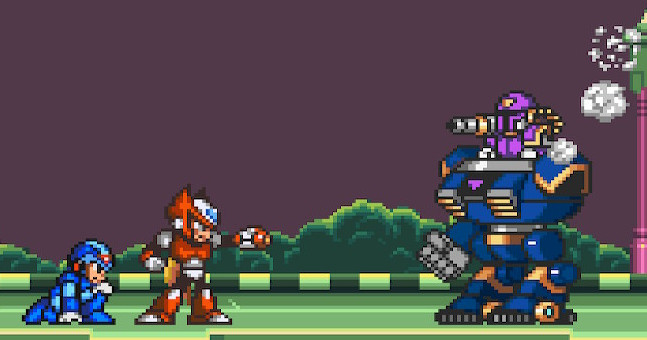
\includegraphics[width=0.5\linewidth]{figures/X1/Highway_end.jpg}
	\caption{Zero saving X from Vile.}
\end{figure}

The couple decides to part ways: Zero embarks on a mission to locate the enemy fortress, while X takes on the task of confronting Sigma's mavericks. As X defeats all eight mavericks, he gains new power-ups and strength along the way. Eventually, he reunites with Zero, who had been searching for the Sigma fortress flying over the sea. However, upon reaching the fortress's entrance, they are immediately faced with Vile and his formidable ride armor. In a one-versus-one battle, Zero courageously challenges Vile but is ultimately captured. Subsequently, Vile also manages to ensnare X, gloating over his apparent triumph. At this critical moment, Zero seizes an opportunity to break free from his confinement. He attaches himself to the ride armor and detonates, destroying the armor but sparing Vile. Witnessing Zero's selfless act of sacrifice, X finds newfound determination, empowering him to break free as well. He confronts Vile, who is now vulnerable, and successfully defeats him in battle.

Before proceeding further, X heeds Zero's final words~\cite{wiki:MMX_script}. Zero reveals to X that his auto-repair system is incapable of handling all the damages he sustained during their battles, while also telling X he possesses a power even greater than his, rendering him capable of facing Sigma (eventually even entrusting his own Z-buster to X in case he had not managed to acquire the buster upgrade himself).

\begin{figure}[htp]
	\centering
	
\includegraphics[width=0.5\linewidth]{figures/X1/Zero_cannon.jpg}
	\caption{Zero, near death, giving X his arm cannon.}
\end{figure}

Following Zero's demise, X continues his mission and infiltrates Sigma's fortress and confronts its dangers, including re-facing all the previously defeated mavericks. Eventually, X arrives at Sigma's lair, where the villain awaits. Sigma initially displays arrogance, being surprised that X managed to reach him and claiming he could easily destroy him. However, Sigma decides to let his pet Velguarder deal with X as he watches the fight unfold. X proves his skill by successfully defeating Velguarder, which changes Sigma's perspective a bit, understanding why Zero placed his trust in X and acknowledging that X could have been an hunter as strong as he was. Sigma then faces X himself, but ultimately X emerges victorious, destroying all Sigma's body but his head. Sigma's head then combines with a giant wolf-based mechaniloid, providing him with a new body to continue the battle against X. Despite Sigma's tenacity, however, X manages to destroy the new body too, effectively putting an end to Sigma. 

Just as the fights end,  the fortress begins to explode, while Sigma blames X for shattering his dream of a world exclusively for reploids. The fortress's imminent destruction forces X to teleport to safety outside. Contemplating the consequences of the destruction he has witnessed and the sacrifices made for victory, X questions if fighting was the right choice, wondering if an alternative path could have been taken. As the flying fortress sinks into the ocean, X realizes that he will face more battles before finding the answers he seeks. The game's credits roll, but an unexpected twist emerges. A message from Sigma reveals that his spirit is still intact, awaiting the construction of a new body to challenge X once again. 
\begin{figure}[htp]
	\centering
	
\includegraphics[width=0.45\linewidth]{figures/X1/Ending.jpg}
	
\includegraphics[width=0.45\linewidth]{figures/X1/sigma_message.jpg}
	\caption{Sigma's fortress falling in the ocean and Sigma's final message to X.}
\end{figure}

\section{Main Plot (\mhx)}
While Maverick Hunter X largely follows a similar plot to the original Mega Man X game, it does introduce some divergences, particularly concerning the relationships between characters and X's background~\cite{wiki:MM_MHX}. One of the significant points of divergence pertains to X's backstory before the commencement of the war. Below is a summary of the differences between \textit{Maverick Hunter X} and Mega Man \x:


\begin{itemize}
	
\item In-depth background: The "``Day of $\Sigma$'' OVA provides a comprehensive background of the war, explaining how Sigma initiated his revolution. In this version, X's background is altered, and he is already a Maverick Hunter before the war's beginning. He serves in the 17th Elite Unit alongside Zero, both commanded by Sigma himself. X holds a B hunter rank, which differs from Zero's SA rank, due to his pacifist nature and preference for dialogue over combat. Many mistake these traits for weakness, but Zero and Sigma recognize X's true potential.

\item Expanded background for Vile: Vile's character receives additional depth in Maverick Hunter X. Here, he aims to destroy both X and Sigma, seeking to create his own world. As a result, he follows Sigma's plans merely because they align with his own objectives.

\item Differences in the final portion of the story: Maverick Hunter X diverges in the final level's layout and story progression~\cite{wiki:MM_MHX_script}. Unlike the original game, where X and Zero immediately confront Vile upon entering Sigma's fortress, here, X first traverses the fortress, encountering previously defeated bosses resurrected to challenge him. Only at the end does X meet with Zero and encounter Vile. As in the main story, Vile captures both of them, leading to Zero's sacrifice and X ultimately defeating Vile.

\item Sigma's attitude toward X: In Maverick Hunter X, Sigma already suspects X's immense potential. He tests X by making him fight Velguarder, rather than assuming Velguarder alone would be enough to defeat X, as in the original game. Sigma then confronts X directly, leading to the same outcome as in the original story.

\end{itemize}

These differences in character backgrounds, relationships, and story progression add new dimensions and complexities to the familiar tale of Mega Man X.

\section{Main Characters}
\subsection{X}
\begin{figure}[htp]
	\centering
	
\includegraphics[width=0.3\linewidth]{figures/X1/X_X1.png}
	\caption{X}
\end{figure}

X, as described in Chapter~\ref{char:X}, is the first of a new generation of sentient robots created by Dr.~Thomas Light in the year 20XX. He possesses the unique ability to experience emotions and make autonomous decisions. Due to X's immense power, Dr.~Light needed to conduct a series of tests to ensure his integrity. Unfortunately, Dr.~Light's own lifespan would not permit him to complete all the tests, so he sealed X in a capsule capable of running autonomous tests.

In the year 21XX, during an archaeological expedition, Dr. Cain (chapter~\ref{char:Cain}) discovers X's capsule~\cite{X:Manual,wiki:Cain_journal}. Dr. Cain reawakens X and, with the aid of Light's designs and X's assistance, develops a new type of robot called ``Reploids''. The Reploids quickly become integrated into society and prove invaluable in performing challenging tasks. Despite this newfound purpose, X remains uncertain about his place in the world and the future that Dr. Light envisioned for him. However, when the villainous Sigma initiates a war against humanity, X is compelled to step forward and fight alongside his ally, Zero, to restore peace.

The account given so far aligns with X's original role in the original game. However, as mentioned earlier, Maverick Hunter X rewrites X's backstory, introducing a different series of events before Sigma's revolt. In this retelling, Dr. Light seals X away not to test his integrity but because he believes the world is not yet ready for X's technology and potential. Dr. Light is steadfast in his belief that X possesses a good spirit and will use his power to achieve peace~\cite{wiki:MM_MHX_X}. Furthermore, upon awakening X joins immediately the Maverick Hunters (a deviation from the original storyline), serving in the 17th Elite Unit alongside Zero under Sigma's direct command. Despite X's extraordinary potential, his hunter rank is designated as B, unlike Zero's SA rank. This lower rank is attributed to X's apparent hesitation during battle, a result of his pacifist nature, which makes him reluctant to fight and prevents him from fully utilizing his true power~\cite{Xcoll1:Manual_X1}. Nevertheless, when Sigma launches his war against humanity, X is compelled to rise to the challenge, fighting alongside Zero to restore peace to the world.

\subsection{Zero}
\begin{figure}[htp]
	\centering
	
\includegraphics[width=0.3\linewidth]{figures/X1/Zero_X1.png}
	\caption{Zero}
\end{figure}

In the original Mega Man X1 game, very little information is provided about Zero (more details in chapter~\ref{char:Zero}), other than the fact that he is a friend of X and the new leader of the Maverick Hunters~\cite{X:Manual}. He holds the highest rank among all hunters who have not sided with Sigma. However, Maverick Hunter X delves deeper into Zero's relationship with X, portraying him as a close friend and mentor to X in the 17th Elite Unit, serving under Sigma and holding an SA hunter rank. Zero is depicted as a resolute fighter who staunchly opposes evil, showing no mercy when facing Mavericks, even if they include Sigma himself~\cite{Xcoll1:Manual_X1}.

Despite these differences in character portrayal, Zero's story remains consistent between both games. He first appears at the end of the highway, rescuing X from Vile's clutches and requesting X to handle Sigma's forces while he searches for the enemy hideout. Later, Zero is spotted at the entrance of Sigma's fortress, acting as a diversion to enable X to infiltrate the fortress undetected. Finally, Zero is present during the ultimate showdown with Vile, where he sacrifices himself to destroy Vile's armor, enabling X to defeat him. In his final moments, Zero imparts crucial words to X, urging him to go and confront Sigma. He even gives X his own Z-buster as a backup, in case X hasn't upgraded his own buster yet.

\section{Game Mechanics}
\textit{Mega Man X}'s gameplay remains true to its original series, offering a 2D hybrid experience combining run'n'gun mechanics with platforming elements where the main protagonist, X, must complete different stages to unlock the final area of the game. Each stage has its own distinct theme and contains specific items to collect. Some of these items may require X to obtain other power-ups first, typically acquired from defeating bosses in the game. At the end of each stage, a boss awaits, and defeating him grants X a new weapon based on one of their attacks. Like in the original series, X can access all the main stages in any order, and each boss has a corresponding ``weak point'' vulnerable to a weapon obtained from defeating another boss. Such weakness can be exploited to deal more damages to the boss, but in some occasion they can also stun them or disabling certain bosses' attacks.

Mega Man X1 introduces several new mechanics that will define the series~\cite{wiki:X1_features}:
\begin{itemize}
	
\item Dash: X can dash and move faster, as well as perform dash-jumps with the leg parts. This mechanic is an evolution of the sliding mechanism from the original series, as it is now tied to a specific button.

\item Wall-jumping: X gains the ability to jump onto walls to climb them, as well as slide down for controlled descent. He can also dash-jump off walls to cover greater distances.

\item Armor parts~[\ref{X1:Armor}]: By discovering Dr. Light's capsules (four in total), X can be upgraded and unlock new powers that aid the player during the game.

\item Sub-Weapon charging~[\ref{X1:sub_weapon}]: With the buster upgrade, X can not only charge his primary X-buster, as in the main series, but he can also charge his other sub-weapons to increase damage or alter their functionality.

\item Heart tanks: In addition to the classical Sub-tank, eight heart tanks are scattered across various stages, one per stage. Picking them up increases X's energy capacity by two, starting from 16 and reaching a maximum of 32~\cite{stratwiki:Heart_tank}.

\item Stage interactions: Although limited, beating certain stages can affect others and change them in some portions
\end{itemize}

\section{Weapons}\label{X1:sub_weapon}
Here is a list of all sub-weapons available in\textit{ Mega Man X}/ \textit{Mega Man Maverick Hunter X} (\cite{MHX:manual}, \cite{wiki:X_weapons}):

\subsection{
\includegraphics[width=12px, height=10px]{figures/X1/weapons/Homig_T.jpg} Homing Torpedo}\label{Homing_torpedo}
When X equips this sub-weapon, he gains the ability to fire up to two torpedoes (three in Maverick Hunter X)~\cite{wiki:Homing_torpedo}. These torpedoes possess the unique characteristic of tracking enemies. As they accelerate, they automatically target the nearest enemy and follow its movements. When charged, X can release a fan of four fish-shaped missiles (six in Maverick Hunter X). These charged missiles exhibit increased speed and attack power, making them more effective homing projectiles against enemies. Players obtain this powerful weapon after defeating Launch Octopus~[\ref{boss:Launch_octopus}].

\begin{figure}[htp]
	\centering
	\begin{subfigure}{0.39\linewidth}
		
\includegraphics[width=\linewidth]{figures/X1/weapons/Homing_torpedo_1.jpg}	
	\end{subfigure}
	\begin{subfigure}{0.3\linewidth}
		
\includegraphics[width=\linewidth]{figures/X1/weapons/Homing_torpedo_2.jpg}	
	\end{subfigure}
	\caption{Homing Torpedo sub-weapon's regular and charged attack.}
\end{figure}

\subsection{
\includegraphics[width=12px, height=10px]{figures/X1/weapons/C_sting.jpg} Chameleon Sting}\label{Chameleon_sting}

The Chameleon Sting, acquired after defeating Sting Chameleon~[\ref{boss:Sting_chameleon}], functions by emitting a single laser that subsequently splits into three directions: forward, up-forward, and down-forward. However, in Maverick Hunter X, the weapon directly emits three lasers, which can be angled diagonally upward and downward and have slightly increased speed. In both versions of the game, when the weapon is charged, X flashes in various rainbow colors, granting him temporary invincibility to all damage (except for instant-kill hazards like pits) for a brief period. In the original game X is unable to switch to any other weapon while the invincibility is active. However, in the remake, he has the freedom to fire with the current weapon and use any other weapon simultaneously~\cite{wiki:Chameleon_sting}. 
\begin{figure}[htp]
	\centering
	\begin{subfigure}{0.35\linewidth}
		
\includegraphics[width=\linewidth]{figures/X1/weapons/Chameleon_sting.jpg}
	\end{subfigure}
	\caption{Chameleon Sting sub-weapon}
\end{figure}

\subsection{
\includegraphics[width=12px, height=10px]{figures/X1/weapons/Rolling_S.jpg} Rolling Shield}\label{Rolling_shield}
After defeating Armored Armadillo~[\ref{boss:Armored_Armadillo}], X acquires the Rolling Shield. With this weapon, X spins energy at high speeds within the X-Buster and launches it as an energy shot that rolls along the ground. The resulting projectile is approximately the same size as X (half its size in Maverick Hunter X) and will continue rolling along the ground until it makes contact with an enemy or disappears after a while. If the shield comes into contact with a wall, it ricochets once and then disappear upon hitting a wall again. Only in Maverick Hunter X, the Rolling Shield possesses the additional abilities to absorb incoming projectiles directed toward it and to take out Mets even when they are hiding~\cite{wiki:Rolling_shield}. 

When charged, X can surround himself with an energy field that eliminates any enemy with less than three hit points upon contact. However, the energy field will disappear upon hitting enemies with more than that amount of life. In the original game, while the charged shield is active, X cannot shoot or change weapons in-game. To change weapons, the player must access the pause menu, causing the shield to disappear.

\begin{figure}[htp]
	\centering
	\begin{subfigure}{0.35\linewidth}
		
\includegraphics[width=\linewidth]{figures/X1/weapons/Rolling_shield_1.jpg}	
	\end{subfigure}
	\begin{subfigure}{0.3\linewidth}
		
\includegraphics[width=\linewidth]{figures/X1/weapons/Rolling_shield_2.jpg}	
	\end{subfigure}
	\caption{Rolling Shield sub-weapon's regular and charged attack.}
\end{figure}

\subsection{
\includegraphics[width=12px, height=10px]{figures/X1/weapons/F_wave.jpg} Fire Wave}\label{Fire_wave}
Fire Wave transforms X's buster into a powerful flamethrower, capable of dealing continuous damage to enemies but which cannot be used underwater. Upon pressing the fire button, X releases a continuous stream of fire from his X-buster, draining energy in the process. When the weapon is fully charged, X launches a fireball that creates a pillar of fire upon hitting the ground, and it moves forward for a certain distance. To charge the weapon, X must continue firing, causing energy to deplete in the process. If used underwater, the weapon becomes ineffective, producing only smoke (but still consuming energy). Players obtain the Fire Wave after defeating Flame Mammoth~[\ref{boss:Flame_mammoth}].

\begin{figure}[htp]
	\centering
	\begin{subfigure}{0.35\linewidth}
		\centering
		
\includegraphics[width=\linewidth]{figures/X1/weapons/Fire_wave_1.jpg}
	\end{subfigure}
	\begin{subfigure}{0.35\linewidth}
		\centering
		
\includegraphics[width=\linewidth]{figures/X1/weapons/Fire_wave_3.jpg}
	\end{subfigure}
\end{figure}
\begin{figure}[htp]
	\ContinuedFloat
	\centering
	\begin{subfigure}{0.34\linewidth}
		\centering
		
\includegraphics[width=\linewidth]{figures/X1/weapons/Fire_wave_2.jpg}
	\end{subfigure}
	\begin{subfigure}{0.36\linewidth}
		\centering
		
\includegraphics[width=\linewidth]{figures/X1/weapons/Fire_wave_4.jpg}
	\end{subfigure}
	\caption{Fire Wave sub-weapon's regular and charged attack both outside and inside water.}
\end{figure}


\subsection{
\includegraphics[width=12px, height=10px]{figures/X1/weapons/Storm_T.jpg} Storm Tornado}\label{Storm_tornado}

The Storm Tornado transforms the X-buster into a powerful fan that unleashes hard-hitting winds, capable of destroying enemies in its path. When fired, it shoots a horizontal tornado that remains on the screen for a brief period before starting to move in the direction X was facing when it was shot. Due to its length, the tornado can hit enemies multiple times, making it an effective way to dispose of most foes, especially larger ones. In Maverick Hunter X, the length of the Storm Tornado is halved, allowing it to shoot at a faster rate.

When the Storm Tornado is charged, it creates a large vortex that covers the entire screen in height. In the original game, this vortex surrounds X himself, while in the remake, it instead explodes from the shot projectile once it hits a solid surface~\cite{wiki:Storm_tornado}. Players obtain the Storm Tornado by defeating Storm Eagle~[\ref{boss:Storm_Eagle}]. 
\begin{figure}[htp]
	\centering
	\begin{subfigure}{0.35\linewidth}
		
\includegraphics[width=\linewidth]{figures/X1/weapons/Storm_tornado_1.jpg}
	\end{subfigure}
	\begin{subfigure}{0.25\linewidth}
		
\includegraphics[width=\linewidth]{figures/X1/weapons/Storm_tornado_2.jpg}
	\end{subfigure}
	\caption{Storm Tornado sub-weapon's regular and charged attack.}
\end{figure}

\subsection{
\includegraphics[width=12px, height=10px]{figures/X1/weapons/E_Spark.jpg} Electric Spark}\label{Electric_spark}
The Electric Spark creates high-pressure voltage within the X-Buster and fires it, allowing for a maximum of three shots at a time. When the electric spark hits a hard surface, it splits in half and starts traveling up and down along the surface.

In the original Mega Man X1, when this weapon is charged, X releases two electric columns in front and behind him, which moves in their respective directions. On the other hand, in Maverick Hunter X, the weapon generates electricity in all directions starting from X's body, covering the entire screen. 

Players obtain the Electric Spark upon defeating Spark Mandrill~[\ref{boss:Spark_mandrill}].

\begin{figure}[htp]
	\centering
	\begin{subfigure}{0.35\linewidth}
		
\includegraphics[width=\linewidth]{figures/X1/weapons/Electric_spark_1.jpg}
	\end{subfigure}
	\begin{subfigure}{0.25\linewidth}
		
\includegraphics[width=\linewidth]{figures/X1/weapons/Electric_spark_2.jpg}
	\end{subfigure}
	\begin{subfigure}{0.3\linewidth}
		
\includegraphics[width=\linewidth]{figures/X1/weapons/Electric_spark_3.jpg}
	\end{subfigure}
	\caption{Electric Spark sub-weapon's regular (normal and split) and charged attack.}
\end{figure}

\subsection{
\includegraphics[width=12px, height=10px]{figures/X1/weapons/B_cutter.jpg} Boomerang Cutter}\label{Boomerang_cutter}

Upon defeating Boomer Kuwanger~[\ref{boss:Boomer_Kuwanger}], X gains access to the Boomerang Cutter. This unique weapon fires up to three sharp boomerangs~\cite{wiki:Boomerang_cutter} made from a special metal. The trajectory of these boomerangs depends on X's position when he fires them: they arc upwards if X is standing on the ground and arc downwards if X is in the air. If a boomerang fails to hit an enemy, it returns to X, and if it passes an item on its way back, it picks up the item and delivers it to X, even retrieving dropped life or weapon energy from defeated enemies. If a boomerang successfully returns to X without hitting an enemy, it replenishes the energy used to create it. When charged, X releases four larger boomerangs that spiral out of him diagonally. In Maverick Hunter X, this has been altered to four boomerangs of doubled size that move back and forth in a straight line a few times.

Additionally, the Boomerang Cutter has a special perk when used against Flame Mammoth and Launch Octopus. While such enemies are not heavily damaged by the weapon, hitting Flame Mammoth will cause hit to lose his trunk, while Launch Octopus will lose his tentacles, resulting in both bosses being unable to perform certain attacks anymore.

\begin{figure}[htp]
	\centering
	\begin{subfigure}{0.3\linewidth}
		
\includegraphics[width=\linewidth]{figures/X1/weapons/Boomerang_1.jpg}
	\end{subfigure}
	\begin{subfigure}{0.3\linewidth}
		
\includegraphics[width=\linewidth]{figures/X1/weapons/Boomerang_2.jpg}
	\end{subfigure}
	\caption{Boomerang Cutter sub-weapon's regular and charged attack.}
\end{figure}

\subsection{
\includegraphics[width=12px, height=10px]{figures/X1/weapons/S_ice.jpg} Shotgun Ice}\label{Shotgun_ice}

Shotgun Ice is the weapon that X acquires after defeating Chill Penguin~[\ref{boss:Chill_Penguin}]. This powerful weapon absorbs moisture from the air and fires it in crystallized form which, upon hitting an enemy or a hard surface, shatter into five pieces that ricochet backward. If these ice fragments collide with another wall or enemy, they are destroyed. When charged, the weapon has a different effect in the original game and its remake. In Mega Man X1 the charged Shotgun Ice creates a Chill Penguin-shaped ice platform, resembling the ice sculpture that the boss can create. X can stand on this platform, and it starts moving forward shortly after being created. However, in Maverick Hunter X, the charged version only creates a sharp sled of ice without the platform's decorative shape.

A notable quirk in Mega Man X1 is that if X creates the platform and then positions himself in the same spot where the platform is forming (due to the platform's delayed creation), the platform will slightly push X left or right based on its position. This can lead to glitches such as wall clipping, allowing X to pass through walls in certain circumstances ~[\ref{X1:misc}]. This glitch is not present in Maverick Hunter X.

\begin{figure}[htp]
	\centering
	\begin{subfigure}{0.3\linewidth}
		
\includegraphics[width=\linewidth]{figures/X1/weapons/Shotgun_ice_1.jpg}
	\end{subfigure}
	\begin{subfigure}{0.31\linewidth}
		
\includegraphics[width=\linewidth]{figures/X1/weapons/Shotgun_ice_2.jpg}
	\end{subfigure}
	\begin{subfigure}{0.29\linewidth}
		
\includegraphics[width=\linewidth]{figures/X1/weapons/Shotgun_ice_3.jpg}
	\end{subfigure}
	\caption{Shotgun Ice sub-weapon's regular (normal and deflected shots) and charged attack.}
\end{figure}

\section{First Armor}\label{X1:Armor}

While exploring stages, X may come across one of the four capsules hidden by Dr. Light. When X comes into contact with a capsule, it opens, revealing Dr.~Light's hologram, which will speak to X and present him with one of the armor parts~\cite{wiki:First_armor}, providing an explanation of how the specific armor part functions. 
\begin{figure}[htp]
	\centering
	
\includegraphics[width=0.2\linewidth]{figures/X1/First_armor.png}
	\caption{First armor X.}
\end{figure}

The First Armor is comprised of four parts (plus an extra one), each offering unique enhancements to X's abilities:
\begin{itemize}
\item \emph{Foot Parts}: The ``\textit{Emergency Acceleration System}''~\cite{X:Manual} allows X to dash forward, perform dash-jumps, and execute wall dash-jumps. While dashing, his hitbox's height is reduced slightly. Additionally, X can destroy specific blocks by wall-jumping onto them. In the original Mega Man X, the capsule containing the foot parts is located in the middle of the Snow Mountain Stage and is mandatory to obtain. However, in Maverick Hunter X, the capsule is moved to the beginning of the Factory Stage.

\item \emph{Body Parts}: Equipping the Body Parts reduces all incoming damage to X by 50\%. In the original game, the capsule is found in the Forest stage after climbing the wall right before the cave. After defeating RT-55J, the capsule will emerge from the ground. In Maverick Hunter X, the Body Parts are moved to the Storm Eagle Stage, requiring the Head Parts to access them.

\item \emph{Arm Parts}: These allow X's X-Buster to be charged up to a third level and enable charging of special weapons. Dr.~Light originally intended this upgrade to be included in the basic X-Buster~\cite{X:Manual}, but he sealed away X before it was ready, making it a separate modification given to X later. While the capsule itself is not mandatory, if the player faces Vile without finding the capsule first, the game will still grant them the buster upgrade in the form of the Z-Buster. In Maverick Hunter X, the Arm Parts unlock the Spiral Crush Buster, which is a larger version of the second-level charged shot and hits multiple times, while the Z-Buster deals more damage against bosses than the previous alternative. In Mega Man X, the capsule is located in the Factory stage, requiring a precise dash-jump and the Head Parts to break some blocks in the ceiling. In the remake, it is in the same place where the Body Parts were in the original game.

\item \emph{Head Parts}: Equipping the Head Parts grants X the ability to break specific blocks with a headbutt and avoid damage from falling rocks in the Forest stage. In the original game, the capsule is found in the Airport stage, hidden behind an obstacle marked with a flammable warning, which can be destroyed simply by shooting at it. In the remake, it is in Chill Penguin's stage, requiring the foot part to break blocks hiding it.

\item \emph{Hadoken}: While not technically a part of the First Armor, it is a hidden bonus stored inside a Light's capsule. This technique allows X to perform the well-known move from Street Fighter by inputting the button combination $\downarrow$ $\searrow$ $\rightarrow$ (with X facing right) + fire button or using the same combination while X is charging and releases the charged shot~\cite{RTA_wiki:X1}, provided that X is at full health. The projectile deals 32 points of damage~\cite{wiki:Hadoken} to all enemies, essentially one-shotting every non-shielded enemy, including bosses. The only exception is Sigma's final form, but this limitation exists only in the original Mega Man X. In both the original game and its remake, the capsule containing the Hadoken is hidden in Armored Armadillo's stage. It's worth noting that in the original game, the Hadoken power-up is not saved by the password system, meaning it has to be unlocked again if the game is restarted. However, in the remake, Maverick Hunter X, this limitation is not present.
\end{itemize}


\section{Highway (Introduction Stage)}

The Highway Stage, also known as Central Highway in \textit{Maverick Hunter X}, serves as the first stage of the game. X arrives here to join the fight against Sigma's forces. The stage serves as a straightforward introduction, where X travels through it while eliminating different enemies and learning basic mechanics like wall-jumping. The stage can be divided into two main sections~\cite{stratwiki:HighWay}, with the second one featuring more hazards such as gaps and falling pieces of the highway (indicated by a darker texture color).

In the first section of the highway, two sub-bosses in the form of \hyperlink{miniboss:Bee_Blader}{Bee Blader} are encountered. At the end of the stage, X faces the \hyperlink{vehicle:Death_Rogumer}{Death Rogumer}, which sends several \hyperlink{enem:Road_Attackers}{Road Attackers} towards him. When some of these enemies are destroyed, Vile appears, dropping from  airship, and starts attacking X with his ride armor. It's important to note that Vile is invincible during this encounter, so fighting back is futile. As X's health drops below a certain threshold, Vile will begin shooting an energy projectile towards X. If the projectile hits X, he becomes trapped, and the fight ends, leading to the cutscene where Zero comes to save X. In speedruns, players use a technique to start the boss fight with low health, which forces Vile to immediately shoot the trapping projectile, effectively skipping the entire fight. However, caution is required, as Vile will continue attacking with his ride armor, potentially defeating the player if not careful.

\begin{figure}[htp]
	\centering
	
\includegraphics[width=0.5\linewidth]{figures/X1/Highway_screenshot.jpg}
	\caption{X facing Vile.}
\end{figure}

This stage contains following enemies~\cite{wiki:Highway}:
\begin{itemize}
	\item \hyperlink{enem:Ball_De_Voux}{Ball De Voux}
	\item \hyperlink{enem:Bomb_Been}{Bomb Been}
	\item \hyperlink{enem:Crusher}{Crusher}
	\item \hyperlink{enem:Gun_Volt}{Gun Volt}
	\item \hyperlink{enem:Jamminger}{Jamminger}
	\item \hyperlink{enem:Road_Attackers}{Road Attackers}
	\item \hyperlink{enem:Spiky}{Spiky }
	\item \hyperlink{miniboss:Bee_Blader}{Bee Blader }
\end{itemize}

After completing the introduction stage, the player is presented with the classic boss selection screen typical of the Mega Man franchise. 

\begin{figure}[htp]
	\centering
	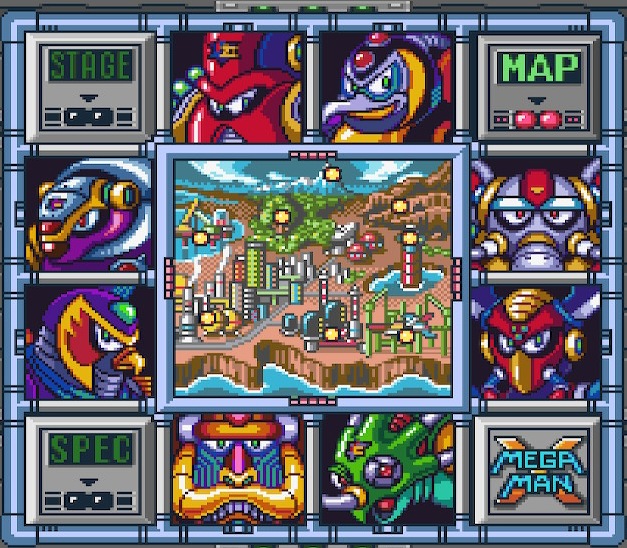
\includegraphics[width=0.5\linewidth]{figures/X1/Full_map.png}
	\caption{Full map with Bosses and their locations}
\end{figure}



\section{Ocean}

The Ocean Stage, later renamed Subterranean Base in \textit{Maverick Hunter X}, is where Launch Octopus hides. The stage begins at the shoreline before X immerses underwater shortly after. Underwater, X gains the ability to jump higher, and skilled players can use this in combination with dash-jumping to skip a significant portion of the stage's first part~\cite{stratwiki:Ocean}. Various fish-based enemies populate the stage, but the main challenges come from the sub-bosses, three in total plus an optional one.

In the first part of the stage, players face difficulties from spiked pits that X must jump over.\hyperlink{enem:Sea_Attacker}{Sea Attackers} will spawn in groups of three from these pits, interrupting X's jumps and potentially causing him to fall into the spikes. Additionally, there are two \hyperlink{miniboss:Anglerge}{Anglerge} sub-bosses that make this section challenging. The second Anglerge is particularly dangerous because it will try to push or pull X into the spiked pits on the floor using its vacuum attack. Players can adopt a strategy of staying on the leftmost platform, shooting, and dashing to the right when the Anglerge starts pulling, then shooting while it pushes X. Anglerges will also shoot serpent-shaped harpoons horizontally, which will then move vertically to hit X when above or below him. Occasionally, they will also shoot a beam of light from their lamp, which can be destroyed.

After passing the second sub-boss, the second part of the stage begins. Here, spiked gaps are less common, but whirlpools appear at regular intervals and specific positions. These whirlpools can propel X up to the ocean's surface. As X proceeds, bombs dropped by a \hyperlink{miniboss:Cruiziler}{Cruiziler} enemy will start falling from above. Players can either climb a whirlpool to get onto the Cruiziler and destroy its core, stopping it from shooting bombs, or they can avoid it and continue through the level. Moving forward, X will encounter an arena filled with sand, where an \hyperlink{miniboss:Utuboros}{Utuboros} will attack by rising from the sand, swimming for a while, and then submerging again. This enemy is invincible for most of its body, with only the head and tail being vulnerable. Although its weakness is considered to be the Boomerang Cutter, players can use the Storm Tornado to destroy it in one shot by firing it from behind its head ~\cite{wiki:Utuboros}. After defeating this sub-boss, and moving forward, X will reach the boss door.

Here is a list of all enemies present in the stage~\cite{wiki:Ocean}:
\begin{itemize}
	\item \hyperlink{enem:Amenhopper}{Amenhopper}
	\item \hyperlink{miniboss:Anglerge}{Anglerge}
	\item \hyperlink{miniboss:Cruiziler}{Cruiziler}
	\item \hyperlink{enem:Gulpfer}{Gulpfer }
	\item \hyperlink{enem:Mega_Tortoise}{Mega Tortoise }
	\item \hyperlink{enem:Sea_Attacker}{Sea Attacker}
	\item \hyperlink{enem:Sky_Claw}{Sky Claw }
	\item \hyperlink{miniboss:Utuboros}{Utuboros}
\end{itemize}

\subsection{Heart Tank}
This stage only hides a heart tank. In order to get it the player must first destroy the Cruizer by reaching the ocean's surface via a whirlpool to destroy its core, avoiding in the process the Sky Claws spawned by the ship. Once destroyed, the Cruizer will sink and  destroy the ocean's floor, revealing a hidden portion with a large room filled with spikes on the ground. Here an Utuboros  must be defeated to open the door which leads to a Heart Tank. 
\begin{figure}[htp]
	\centering
	\begin{subfigure}{0.4\textwidth}
		\centering
		
\includegraphics[height=3cm]{figures/X1/Launch_octopus/Octopus_heart_1.jpg}
		\caption{}
	\end{subfigure}
	\begin{subfigure}{0.4\textwidth}
		\centering
		
\includegraphics[height=3cm]{figures/X1/Launch_octopus/Octopus_heart_2.jpg}
		\caption{}
	\end{subfigure}
	\begin{subfigure}{0.4\textwidth}
		\centering
		
\includegraphics[height=3cm]{figures/X1/Launch_octopus/Octopus_heart_3.jpg}
		\caption{}
	\end{subfigure}
	\caption{(a)Via whirlpool the player can reach the Cruizer on ocean's surface,(b) When destroyed the ship will fall and break the ocean floor (c) Once destroyed the Utuboros inside the cave, a room will open with the Heart Tank inside}
\end{figure}

\begin{figure}[htp]
	\centering
	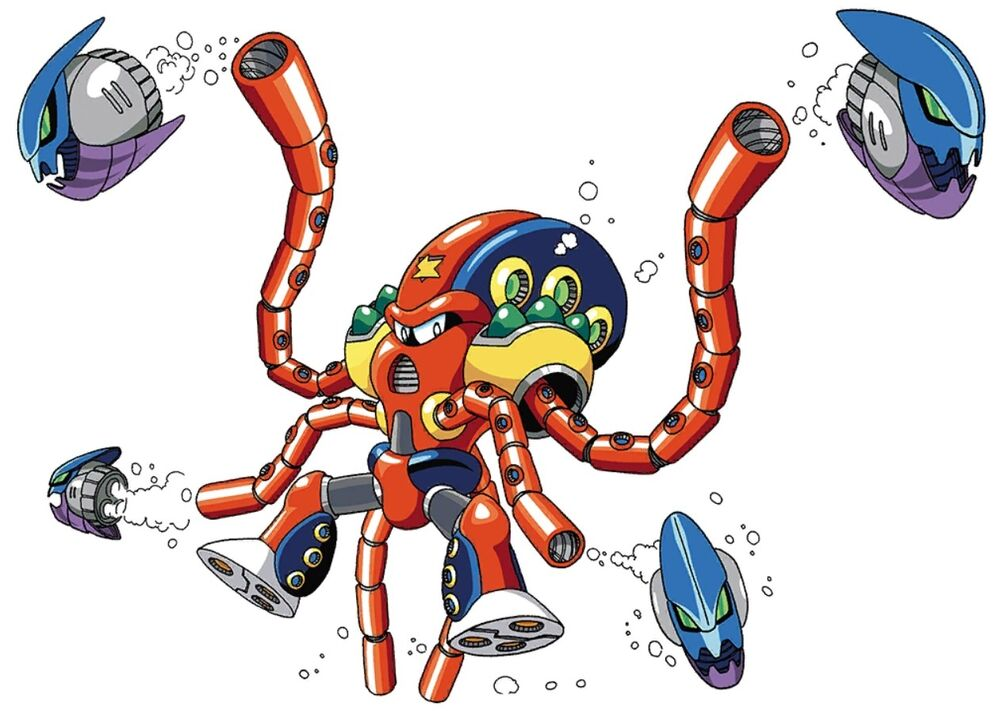
\includegraphics[height=5cm]{figures/X1/Launch_octopus/LaunchOctopus.jpg}
	
\includegraphics[height=5cm]{figures/X1/Launch_octopus/MHXLaunchOctopus.jpg}
	\caption{Launch Octopus' designs (\cite{book:MMX_Complete_art})}
\end{figure}

\subsection{Launch Octopus}\label{boss:Launch_octopus}

Launch Octopus, also known as the ``\textit{General of the Deep Sea}''~\cite{book:MMX_Complete_art} was originally a Maverick Hunter of the 6th Fleet armada before joining Sigma's rebellion and setting his base in the dept of the Ocean, in order to attack marine cities and cut off shipping routes. In the original Mega Man X game, he sided with Sigma because he shared the dream of a world only for reploids and was dubious about protecting humans. However, in Maverick Hunter X, he is portrayed as a military tactician who seeks beauty in combat and considers himself an unappreciated artist of underwater fighting. Only Sigma understood his art, leading Launch Octopus to join him~\cite{wiki:MM_MHX_script}.

\begin{figure}[htp]
	\centering
	\begin{subfigure}{0.48\textwidth}
		\centering
		
\includegraphics[width=\linewidth]{figures/X1/Launch_octopus/Octopus_missile.jpg}
		\caption{Homing Torpedo}
	\end{subfigure}
	\begin{subfigure}{0.49\textwidth}
		\centering
		
\includegraphics[width=\linewidth]{figures/X1/Launch_octopus/Octopus_piranha.jpg}
		\caption{Charged Homing Torpedo}
	\end{subfigure}
\end{figure}
\begin{figure}
	\ContinuedFloat
	\centering
	\begin{subfigure}{0.2\textwidth}
		\centering
		
\includegraphics[width=\linewidth]{figures/X1/Launch_octopus/Octopus_vortex.jpg}
		\caption{Vortex}
	\end{subfigure}
	\begin{subfigure}{0.37\textwidth}
		\centering
		
\includegraphics[width=\linewidth]{figures/X1/Launch_octopus/Octopus_drain.jpg}
		\caption{Energy Drain}
	\end{subfigure}
	\begin{subfigure}{0.39\textwidth}
		\centering
		
\includegraphics[width=\linewidth]{figures/X1/Launch_octopus/Octopus_cut.jpg}
		\caption{Tentacles cut off}
	\end{subfigure}
	\caption{Launch Octopus' attacks}
\end{figure}
During the boss battle, Launch Octopus has three main techniques: the Homing Torpedo, a charged version of the previous attack (which is faster and more powerful), and the Energy Drain.  Octopus often starts the fight with a barrage of homing missiles, to then switches to one of his other two attacks. Notably all version of his homing missiles can be destroyed by shooting at them. His Energy Drain attack involves him swimming in the upper left or right corner, spinning to create a whirlpool to suck X in and drain his energy to replenish his own.

Octopus main weakness is the Rolling Shield, which deals extra damage to him. The Boomerang Cutter is also effective weapon, as it can sever his tentacles in three hits, preventing him from using his Energy Drain attack. Upon defeating Launch Octopus, X gains the Homing Torpedo weapon (\ref{Homing_torpedo}). Additionally, this victory causes a flood in the Forest Stage, resulting in water appearing near the beginning of that stage.

In terms of his official measurements, Launch Octopus is listed as 232 cm tall and 182 kg heavy\cite{wayback:X_resources}, though there may be discrepancies between in-game information and the official data~\cite{wiki:Launch_octopus}


\begin{figure}[htp]
	\begin{minipage}[c]{0.45\linewidth}
		\vspace{0pt}
		\centering
		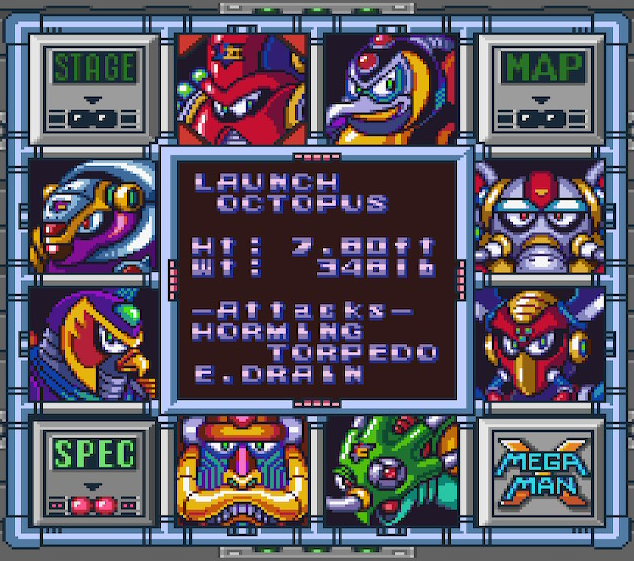
\includegraphics[width=\linewidth]{figures/X1/Launch_octopus/Launch_octopus_specs.png}
	\end{minipage}
	\begin{minipage}[c]{0.45\linewidth}
		\centering
		\vspace{0pt}
		\begin{tabular}[h]{l c}
			\toprule
			Health Bar & 32\\
			\midrule
			\multicolumn{1}{c}{Attack} & \multicolumn{1}{c}{Damage}\\
			Contact & 4\\
			Homing Torpedo & 2\\
			Charged H. Torpedo & 2\\
			Energy Drain & 1-15\\
			\bottomrule
		\end{tabular}
	\end{minipage}
	\caption{Left: Launch Octopus' specifications and according to X1; Right: In-game data~\cite{wiki:Launch_octopus}. }
	\label{Octopus_specs}
\end{figure}


\section{Snow Mountain}

Snow Mountain, also known as the \textit{Abandoned Missile Base} in Maverick Hunter X, is often the first stage that many players choose when starting the game due to its relatively low level of danger~\cite{stratwiki:Snow_mountain} and the valuable upgrade it contains—the Foot Parts. The stage is set in a snow-covered mountain that X must climb to reach the boss.

The stage can be divided into three main areas. In the first area, X starts outside and follows a path that leads him into a cave while encountering various enemies along the way. Inside the cave (the second area), X must climb while avoiding enemies dropping from higher levels. He also needs to navigate across frozen platforms separated by pits until he reaches the end of the cave. In the third area, X returns to the outside and has the option to use a Ride Armor. With the Ride Armor, he can proceed for a while, but he will also face another enemy Ride Armor. The player can choose to keep the Ride Armor and enter a small cave, where they must jump some gaps using the armor while dealing with enemies, or they can use the Ride Armor to reach the top of the cave by jumping out of it to gain extra lift, effectively skipping the lower portion.

Afterwards, there is a tall wall that the Ride Armor cannot surpass, and X must leave it behind. Here, he follows a path full of slopes, gaps, and \hyperlink{enem:Snow_Shooter}{Snow Shooters}, which throw snowballs that become larger the longer they roll on the snowy ground. After passing these obstacles, the player will reach the boss door, where they will face the stage's boss.

The stage contains following enemies~\cite{wiki:Snow_mountain}:
\begin{itemize}
	\item \hyperlink{enem:Armor_Soldier}{Armor Soldier} (with Ride Armor)
	\item \hyperlink{enem:Axe_Max}{Axe Max}
	\item \hyperlink{enem:Batton_Bone}{Bat Bone}
	\item \hyperlink{enem:Bomb_Been}{Bomb Been}
	\item \hyperlink{enem:Flammingle}{Flammingle}
	\item \hyperlink{enem:Jamminger}{Jamminger }
	\item \hyperlink{enem:Ray_Bit}{Ray Bit}
	\item \hyperlink{enem:Snow_Shooter}{Snow Shooter}
	\item \hyperlink{enem:Spiky}{Spiky}
	\item \hyperlink{enem:Tombot}{Tombot}
\end{itemize}

\subsection{Light's Capsule}\label{X:Foot_Parts}

In the original Mega Man X, the Snow Mountain stage contains the Armor capsule for the Foot Parts. This upgrade allows X to dash, perform dash-jumps, and execute wall dash-jumps. Dashing also reduces X's height and hitbox slightly, enabling him to dodge certain attacks by dashing beneath them. The capsule is conveniently located directly on the main path after climbing the first part of the cave. Since it is placed right in the middle of the path, it cannot be avoided, making it the only mandatory capsule in the entire series.
\begin{figure}[htp]
	\centering
	
\includegraphics[width=0.5\textwidth]{figures/X1/Chill_penguin/Armor_foot.jpg}
	\caption{Foot Part capsule location}
\end{figure}

However, in the remake, Mega Man Maverick Hunter X (MHX), the Snow Mountain stage hides the Head Parts instead. The capsule for the Head Parts is concealed in the first indoor climbing section and can only be accessed by breaking a block that requires the use of the Foot Parts.


\subsection{Heart Tank}\label{Penguin:heart_tank}

The stage's, Heart Tank is hidden in the last igloo X encounters before facing the section with snowballs, and to reach it X must use the Ride Armor. Passed the first igloo, there is a light blue column located just before the cave with the enemy Ride Armor,  from the top of which the player must jump with the Ride Armor and, at the maximum height, jump out of it to reach the wall leading to the upper path. On this upper path two other igloos can be found, which can be destroyed using the Fire Wave weapon. Among these igloos, the last one contains the Heart Tank that the player is seeking to collect

\begin{figure}[htp]
	\centering
	\begin{subfigure}{0.375\linewidth}
		\centering
		\includegraphics[width=\textwidth]{figures/X1/Chill_penguin/Chill_heart_1.jpg}	
		\caption{}
	\end{subfigure}
	\begin{subfigure}{0.4\linewidth}
		\centering
		\includegraphics[width=\textwidth]{figures/X1/Chill_penguin/Chill_heart_2.jpg}	
		\caption{}
	\end{subfigure}
	\caption{Heart Tank location.}
\end{figure}

\subsection{Chill Penguin}\label{boss:Chill_Penguin}
\begin{figure}[htp]
	\centering
	\includegraphics[height=5cm]{figures/X1/Chill_penguin/Chill_Penguin.jpg}
	\includegraphics[height=5cm]{figures/X1/Chill_penguin/MHXChillPenguin.jpg}
	\caption{Chill Penguin's designs (~\cite{book:MMX_Complete_art})}
\end{figure}

Chill Penguin, also known as the ``\textit{Glacial Emperor}''~\cite{book:MMX_Complete_art} was originally part of the 13th Polar Division, specifically designed to operate in polar environments due to his small size. However, due to the long permanence away from civilization, he grew tired of his mission in the South Pole and sought a way to escape. When Sigma's rebellion began, it provided Chill Penguin with the opportunity he needed to leave the South Pole and join Sigma's cause. In Mega Man X1, Chill Penguin eliminated his own commander and took over a mountain base to cause chaos with avalanches~\cite{Xcoll1:Manual_X1}, while in \textit{Maverick Hunter X}, it was Sigma who brought Chill Penguin out of the South Pole and enlisted him in the 17th division~\cite{MHX:manual} before declaring war, alongside a payment to ensure Penguin's loyalty to his army~\cite{wiki:MMX_script}. He  was known to be a belligerent and rowdy individual, sometimes showing jealousy towards Flame Mammoth and his size (\ref{boss:Flame_mammoth}).

\begin{figure}[htp]
	\centering
	\begin{subfigure}{0.44\textwidth}
		\centering
		\includegraphics[width=\linewidth]{figures/X1/Chill_penguin/Chill_shot.jpg}
		\caption{Shotgun Ice}
	\end{subfigure}
	\begin{subfigure}{0.53\textwidth}
		\centering
		\includegraphics[width=\linewidth]{figures/X1/Chill_penguin/Chill_frozen.jpg}
		\caption{X frozen near two ice statues}
	\end{subfigure}
	\begin{subfigure}{0.5\textwidth}
		\centering
		\includegraphics[width=\linewidth]{figures/X1/Chill_penguin/Chill_shatter.jpg}
		\caption{Chill Penguin's shotgun ice stopped by his own statues}
	\end{subfigure}
	\begin{subfigure}{0.4\textwidth}
		\centering
		\includegraphics[width=\linewidth]{figures/X1/Chill_penguin/Chill_slide.jpg}
		\caption{Slide attack}
	\end{subfigure}
	\begin{subfigure}[t]{0.5\textwidth}
		\centering
		\includegraphics[width=\linewidth]{figures/X1/Chill_penguin/Chill_blizzard.jpg}
		\caption{Blizzard attack}
	\end{subfigure}
	\begin{subfigure}[t]{0.35\textwidth}
		\centering
		\includegraphics[width=\linewidth]{figures/X1/Chill_penguin/Chill_burn.jpg}
		\caption{Chill Penguin is burnt by the Fire Wave}
	\end{subfigure}
	\caption{Chill Penguin's attacks}
\end{figure}

Chill Penguin is often considered the easiest boss of the game and the first one a player should face due the simplicity of avoiding his attacks, also thanks to the Foot Parts the stage gives to the player. He has four main attacks which he performs at random~\cite{wiki:Chill_Penguin}. When using his Shotgun Ice, Chill Penguin will shoot four frozen projectiles which travel in a straight line, although some of them  can fall off and slide on the ground, that shatter upon contact with a wall and can nullify X's shots when two meet. Other times instead of his projectiles he will emit a snowy breath which will create two penguin-shaped ice sculptures and freeze X if he is in the breath's range. The sculptures act both as obstacles that damage X and as covers since they blocks all projectiles, and require few shots to destroy them. 

On some occasion Chill Penguin will leap in the air and grab the hook on the ceiling, unleashing a blizzard which will push X and the statues (if present) against a wall, causing sculptures to shatter in the process. Finally he can also slide on the floor, and bounce back if he hits a wall. While in this state he is invincible, but he also gets rid of the remaining sculptures.  

Since Chill Penguins attacks only cover the low part of the arena,  the best strategy use against him consists in staying on the higher ground part via continuous wall-jumps, dropping down only to hit him when vulnerable. The catch here is that sometimes Chill Penguin will perform a high jump toward X, hitting him even if he's in the high corner of the room. 

Chill Penguin's weakness is the Fire Wave, which burns and stuns him temporarily. After defeating him, X gains the Shotgun Ice weapon (\ref{Shotgun_ice}) while causing also  the lava in the Factory Stage to get frozen, making the stage less dangerous.

Chill Penguin stands at 163 cm tall and weighs 108 Kg, despite some discrepancies in the in-game information screen(\ref{Penguin_specs}).

\begin{figure}[htp]
	\begin{minipage}[c]{0.45\linewidth}
		\vspace{0pt}
		\centering
		\includegraphics[width=\linewidth]{figures/X1/Chill_penguin/Chill_penguin_specs.jpg}
	\end{minipage}
	\begin{minipage}[c]{0.45\linewidth}
		\centering
		\vspace{0pt}
		\begin{tabular}[h]{l c}
			\toprule
			Health Bar & 32\\
			\midrule
			\multicolumn{1}{c}{Attack} & \multicolumn{1}{c}{Damage}\\
			Contact & 6\\
			Shotgun Ice & 2\\
			Ice Breath & 0\\
			Ice statue & 4\\
			Sliding & 6\\
			\bottomrule
		\end{tabular}
	\end{minipage}
	\caption{Left: Chill Penguin's specifications and according to X1; Right: In-game data~\cite{wiki:Chill_Penguin}. }
	\label{Penguin_specs}
\end{figure}


\section{Gallery}
The Gallery Stage, also known as the \textit{Energy Mines Ruins}, is controlled by Armored Armadillo. The stage features mine carts on which X can stand and which, as soon as he boards them, they start moving along the track, increasing in speed and destroying enemies that come into contact with them. However, the player must be careful as all the carts eventually fall into pits, so X needs to jump off at the right moment to avoid falling with them. This stage is known for containing the secret Light's capsule, where X learns the Hadoken technique. It is also a good place to farm health capsules and lives.

The level itself is relatively straightforward. At the beginning, X can ride a mine cart that carries him forward and takes care of enemies until it reaches a series of gaps. After this sequence, a few small gaps and enemies stand between X and the next section, which starts with a long pit where a \hyperlink{miniboss:Mole_Borer}{Mole Borer} emerges from the left wall and chases X. The Mole Borer is invincible, and touching its roller can instantly defeat X. Players can either escape to the right to continue in the level or quickly wall jump to the left before the Mole Borer breaks the wall, and then follow it from behind (while gaining access to the sub-tank). The second part of the stage mirrors the first, with another mine cart ride at the beginning and another Mole Borer at the end. This time, X will land behind the Mole Borer and has to follow it as it creates a passage in the mine. The final cart ride takes the player through remaining enemies until it reaches an opening in the mountain, where it flies over a huge gap that X cannot jump across. To proceed, the player must jump off the cart to land on the other side of the pit (or grab the wall if high enough) and reach the boss door.

Following enemies are present in the stage~\cite{wiki:Gallery}:
\begin{itemize}
	\item \hyperlink{enem:Batton_Bone}{Bat Bone} 
	\item \hyperlink{enem:Batton_M-501}{Batton M-501} 
	\item \hyperlink{enem:Dig_Labour}{Dig Labour} 
	\item \hyperlink{enem:Flammingle}{Flammingle} 
	\item \hyperlink{enem:Metal_Wing}{Metal Wing} 
	\item \hyperlink{enem:Metall_C-15}{Metall C-15} 
	\item \hyperlink{miniboss:Mole_Borer}{Mole Borer}
	\item \hyperlink{enem:Spiky}{Spiky}
\end{itemize}


\begin{figure}[htp]
	\centering
	\includegraphics[width=0.5\linewidth]{figures/X1/Armored_armadillo/Armadillo_tank.jpg}
	\caption{Gallery stage's subtank location}
\end{figure}

\subsection{Sub Tank}
This stage's Sub Tank is located where the first Mole Borer appears. In order to get it the player must jump into the first gap and then immediately wall-jump to the left, in order to let the Mole Borer break the wall pass beneath X. Once it has passed, the player can safely jump off and go left to find the sub tank where the Mole Borer originally was. 

\subsection{Heart Tank}
The heart tank of this stage is located near where the second Mole Borer is found. Once  X jumps off the gap he has to chase the mechaniloid and destroy it quickly, since as it proceeds it will destroy the walls needed to access to the Heart Tank. To do this the Fire Wave weapon is best option, as it deals massive amounts of damage to it in a short amount of time. 
\begin{figure}[htp]
	\centering
	\begin{subfigure}{0.3\linewidth}
		\centering
		\includegraphics[width=\linewidth]{figures/X1/Armored_armadillo/Armadillo_heart.jpg}
		\caption{}
	\end{subfigure}
	\begin{subfigure}{0.3\textwidth}
		\centering
		\includegraphics[width=\linewidth]{figures/X1/Armored_armadillo/Armadillo_heart_2.jpg}
		\caption{}
	\end{subfigure}
	\caption{Gallery stage's heart tank location. In (a) the Mole Borer has been destroyed and X can wall jump and reach it, while in (b) the Mole Borer has passed and X cannot reach the opening anymore}
\end{figure}

\subsection{Hadoken}\label{hadoken}
\begin{figure}[htp]
	\centering
	\includegraphics[width=0.3\linewidth]{figures/X1/Armored_armadillo/Armadillo_hadoken.jpg}
	\caption{Hadoken capsule with Dr.Light in Ryu's attire.}
\end{figure}
The hadoken is the last upgrade X can get before facing the finals stages. The capsule containing it can be unlocked only if the player has managed to collect every other upgrade in the game: eight Heart Tanks, four Sub-Tank, four armor capsules and all the weapons from bosses. 

The best way to make the capsule spawn is as follow: First the player must reach the zone where a single \hyperlink{enem:Batton_M-501}{Batton M-501} drops from the roof  and should farm life-ups by repetitively killing that enemy for at least five lives. Then the player must proceed in the level until the last cart. Here X has to release a charged Sting Chameleon first and immediately after ride the cart until over the pit, jump off to grab the ledge over the boss door, reach its top and jump down into the pit, losing a life and respawning at the last checkpoint. This procedure must be  repeated three more times until, at the  fourth one and if the player reaches the end at full health, the capsule will be there. In the remake the capsule does not require multiple travel through the stage, being available immediately. Once opened, the capsule will reveal Dr. Light wearing Ryu's robes from the Street Fighter series, which will ask X to step into the capsule to teach him the technique. In the Japanese  script of the game~\cite{wordpress:X_japanese_script} Light states that he trained a lot under the nearby waterfall to learn it and, in the remakes, also adds that X is able to learn it due having a nearly-human soul.

\subsection{Armored Armadillo}\label{boss:Armored_Armadillo}
\begin{figure}[htp]
	\centering
	\includegraphics[height=5cm]{figures/X1/Armored_armadillo/Armored_armadillo.jpg}
	\includegraphics[height=5cm]{figures/X1/Armored_armadillo/MHXArmoredArmadillo.png}
	\caption{Armored Armadillo's designs (~\cite{book:MMX_Complete_art})}
\end{figure}
Armored Armadillo, the ``\textit{Armored Warrior}''~\cite{book:MMX_Complete_art} was the commander in charge of the 8th armored force and a soldier loyal to his superior, Sigma. When Sigma started his revolt, Armadillo followed his orders without questioning and occupied a mine to extract raw materials for Sigma's plans of creating weapons.
\begin{figure}[htp]
	\centering
	\begin{subfigure}{0.45\textwidth}
		\centering
		\includegraphics[height=4cm]{figures/X1/Armored_armadillo/Armadillo_rolling.jpg}
		\caption{Rolling Shield}
	\end{subfigure}
	\begin{subfigure}{0.45\textwidth}
		\centering
		\includegraphics[width=\linewidth]{figures/X1/Armored_armadillo/Armadillo_cannon.jpg}
		\caption{Rapid-fire shot}
	\end{subfigure}	
	\begin{subfigure}{0.45\textwidth}
		\centering
		\includegraphics[height=4cm]{figures/X1/Armored_armadillo/Armadillo_energy_1.jpg}
		\caption{Guarding}
	\end{subfigure}
	\begin{subfigure}{0.45\textwidth}
		\centering
		\includegraphics[height=4cm]{figures/X1/Armored_armadillo/Armadillo_energy_2.jpg}
		\caption{Releasing the energy}
	\end{subfigure}
	\begin{subfigure}{0.45\textwidth}
		\centering
		\includegraphics[height=4cm]{figures/X1/Armored_armadillo/Armadillo_shock_1.jpg}
		\caption{Hit by the Electric Spark}
	\end{subfigure}
	\begin{subfigure}{0.45\textwidth}
		\centering
		\includegraphics[height=4cm]{figures/X1/Armored_armadillo/Armadillo_shock_2.jpg}
		\caption{Armor broken}
	\end{subfigure}
	\caption{Armored Armadillo's attacks.}
\end{figure}

Armadillo's fighting style revolves around his impenetrable armor, which he uses both as a shield to deflect X's shots and as a weapon to crush him while using his main attack, the Rolling Shield. In this attack Armadillo turns into a ball and bounces off the arena's walls while being immune to any attack. Between two consecutive rolling shield he will also take out the cannon hidden in his forehead to shoot a rapid sequence of bullets (Rapid-fire shot~\cite{book:Compendium}) in a straight line before resuming rolling. Additionally, Armored Armadillo can also guard against X's attacks, making himself invincible while absorbing and re-releasing charged shots fired at him.
The main challenge in fighting Armored Armadillo is finding the right moments to attack him when he is vulnerable, as he becomes invincible while rolling. However, the Electric Spark, his weak point, helps in this regards, as it deals extra damage to him while also removing his armor. Once his armor is gone, Armadillo loses the ability to guard and his invincibility while rolling, thus becoming easier to defeat.
\begin{figure}[htp]
	\begin{minipage}[c]{0.45\linewidth}
		\vspace{0pt}
		\centering
		\includegraphics[width=\linewidth]{figures/X1/Armored_armadillo/Armored_armadillo_specs.png}
	\end{minipage}
	\begin{minipage}[c]{0.45\linewidth}
		\centering
		\vspace{0pt}
		\begin{tabular}[h]{l c}
			\toprule
			Health Bar & 32\\
			\midrule
			\multicolumn{1}{c}{Attack} & \multicolumn{1}{c}{Damage}\\
			Contact & 6\\
			Rolling Shield& 6\\
			Guarding & 6\\
			Head Beam & 4\\
			\bottomrule
		\end{tabular}
	\end{minipage}
	\caption{Left: Armored Armadillo's specifications and according to X1; Right: In-game data~\cite{wiki:Armored_Armadillo}. }
	\label{Armadillo_specs}
\end{figure}
After defeating Armored Armadillo, X gains the Rolling Shield weapon (\ref{Rolling_shield}), which can be used to overcome certain obstacles and defeat other bosses weak against it. There are no other effects in other stages upon defeating him.

According to the information given, Armored Armadillo is 194 cm tall and 232 kg heavy, but in-game information reports slightly different values (\ref{Armadillo_specs})


\section{Factory} 
The Factory Stage, also known as the \textit{Prototype Weapons Plant} in \textit{MHX}, is one of the more challenging stages among the eight. It takes place inside a factory designated for weapons production, filled with various dangers that can instantly kill X. However if X manages to defeat Chill Penguin before entering the Factory Stage, the molten metal in the level will become frozen solid, reducing the danger significantly as he becomes able to stand on it if he falls from a conveyor belt.
\begin{figure}[htp]
	\centering
	\begin{subfigure}{0.49\textwidth}
		\centering
		\includegraphics[width=\linewidth]{figures/X1/Flame_mammoth/Flame_fire.jpg}
		\caption{}
	\end{subfigure}
	\begin{subfigure}{0.465\textwidth}
		\centering
		\includegraphics[width=\linewidth]{figures/X1/Flame_mammoth/Flame_frozen.jpg}
		\caption{}
	\end{subfigure}\\
	\caption{Factory Stage before (a) and after (b)  defeating Chill Penguin}
\end{figure}
The level is divided into four main parts. The beginning section features two sets of conveyor belts which can hinder X's movement. \hyperlink{enem:Scrap_Robo}{Scrap Robos} constantly spawn on the conveyor belts, either crawling towards X or shooting lasers at him. The next section is a single large room without any conveyor belts. Multiple platforms are at different heights, from which enemies will attack X. This section contains most of the stage's power-ups. Following that is another section with conveyor belts, but this time with dangerous presses that can instantly kill X if he gets caught by them. Careful timing and movement are required to pass through this area unharmed. Finally, the last part of the stage has X walking on pipes with molten iron dripping from them, causing damage but not instant death. There are ladders in this section, but they serve more as side-paths to potentially skip enemies rather than offering significant advantages. At the end of this last section players will find the boss door leading to Flame Mammoth.

These enemies appears in this stage~\cite{wiki:Factory}:
\begin{itemize}
	\item \hyperlink{enem:Dig_Labour}{Dig Labour} 
	\item \hyperlink{enem:Hoganmer}{Hoganmer}
	\item \hyperlink{enem:Metall_C-15}{Metall C-15}
	\item \hyperlink{enem:Scrap_Robo}{Scrap Robo}
	\item \hyperlink{enem:Sky_Claw}{Sky Claw}
	\item \hyperlink{enem:Rolling_Gabyoall}{Rolling Gabyoall}
\end{itemize}

\subsection{Light's Capsule}
Near the big room's entrance players will notice some breakable blocks on the roof . To access this area, X needs to have obtained the Head Part and the Foot Parts. To reach the capsule, the player needs to perform a precise dash-jump to the left from the very end of the first platform, causing X to destroy the rightmost block and creating a foothold to perform a wall-jump. The player must continue wall-jumping to climb upward while breaking the remaining blocks to reach the capsule with the Arm Parts. If X destroys the first block but fails to start the wall-jump it is still possible to recover, but the jump becomes even more difficult, although doable with enough precision. If the player accidentally destroys the second block as well, it becomes impossible to climb up to the capsule, and the player must sacrifice X to reset the area.

In the Maverick Hunter X remake, the capsule is easier to access since the roof is lower, requiring no other items to reach it. However, this time the capsule contains the Foot Parts instead.
\begin{figure}[htp]
	\centering
	\begin{subfigure}{0.4\textwidth}
		\centering
		\includegraphics[height=3cm]{figures/X1/Flame_mammoth/Flame_armor_1.jpg}
		\caption{}
	\end{subfigure}
	\begin{subfigure}{0.4\textwidth}
		\centering
		\includegraphics[height=3cm]{figures/X1/Flame_mammoth/Flame_armor_2.jpg}
		\caption{}
	\end{subfigure}\\
	\caption{Buster upgrade position: a dash-jump is required from (a) to to start wall-jumping and break the ceiling to reach (b).}
\end{figure}

\subsection{Sub Tank}
In the big room, while going for the top-right corner brings to the exit, going to the top-left corner will bring the player to the sub tank. To obtain it the player has first to reach the highest platform (the one with a life up) and then dash-jump to the left to reach the wall and climb it. While climbing X will reach a part of the wall made of block breakable with the Foot Parts. Behind these blocks there is a small path with the sub tank in it.
\begin{figure}[htp]
	\centering
	\includegraphics[height=4cm]{figures/X1/Flame_mammoth/Flame_tank.jpg}
	\caption{Flame Mammoth's Sub Tank}
\end{figure}

\subsection{Heart Tank}
As with  previous power-ups, the Heart Tank too is ``hidden'' in the big room. In truth it isn't hidden at all, since it is in plain sight at the bottom-right corner of the room, floating on top of the molten iron. There is no way X can get it with the iron in the molten state, so the only way to get it is to defeat Chill Penguin first, freezing the ground and allowing X to walk to reach the Heart Tank safely.

\begin{figure}[htp]
	\centering
	\begin{subfigure}{0.49\textwidth}
		\centering
		\includegraphics[width=\linewidth]{figures/X1/Flame_mammoth/Flame_heart_1.jpg}
		\caption{}
	\end{subfigure}
	\begin{subfigure}{0.4\textwidth}
		\centering
		\includegraphics[width=\linewidth]{figures/X1/Flame_mammoth/Flame_heart_2.jpg}
		\caption{}
	\end{subfigure}\\
	\caption{Factory Stage's Heart Tank location. To get it, defeating Chill Penguin is mandatory.}
\end{figure}

\subsection{Flame Mammoth}\label{boss:Flame_mammoth}
\begin{figure}[htp]
	\centering
	\includegraphics[height=5cm]{figures/X1/Flame_mammoth/Flame_mammoth.jpg}
	\includegraphics[height=5cm]{figures/X1/Flame_mammoth/MHXFlameMammoth.jpg}
	\caption{Flame Mammoth's designs (~\cite{book:MMX_Complete_art})}
\end{figure}

Flame Mammoth, known as the ``\textit{Blazing Oil Tank}''~\cite{book:MMX_Complete_art} was once the captain of the 4th Land battalion based in the Middle East before joining Sigma's rebellion and becoming a Maverick. He took great pride in his large size and firepower, which made him arrogant and cocky. Flame Mammoth had a reputation for bullying and humiliating smaller reploids~\cite{wayback:X_resources} (sometimes even hating them~\cite{wayback:X_resources}), such as Chill Penguin~\cite{wiki:Flame_mammoth}. His ultimate desire was to show off his full power and go on a violent rampage, destroying everything he wants, and Sigma's rebellion gave him the perfect occasion to fulfill such desires. After joining Sigma's army alone, as none of his former subordinates wanted to follow their hated leader~\cite{MHX:manual}, Mammoth was put in charge to defend the weapon factory supplying Sigma's army.

\begin{figure}[htp]
	\centering
	\begin{subfigure}{0.4\textwidth}
		\centering
		\includegraphics[width=\linewidth]{figures/X1/Flame_mammoth/Mammoth_oil.jpg}
		\caption{Oiling}
	\end{subfigure}
	\begin{subfigure}{0.4\textwidth}
		\centering
		\includegraphics[width=\linewidth]{figures/X1/Flame_mammoth/Mammoth_fire.jpg}
		\caption{Fire Wave}
	\end{subfigure}\\
	\begin{subfigure}{0.5\textwidth}
		\centering
		\includegraphics[width=\linewidth]{figures/X1/Flame_mammoth/Mammoth_oil_fire.jpg}
		\caption{Oil ignited by the fire}
	\end{subfigure}
	\begin{subfigure}{0.3\textwidth}
		\centering
		\includegraphics[width=\linewidth]{figures/X1/Flame_mammoth/Mammoth_trunk.jpg}
		\caption{Trumpet}
	\end{subfigure}
	
	\begin{subfigure}{\textwidth}
		\centering
		\includegraphics[width=0.3\linewidth]{figures/X1/Flame_mammoth/Mammoth_press_1.jpg}
		\includegraphics[width=0.4\linewidth]{figures/X1/Flame_mammoth/Mammoth_press_2.jpg}
		\caption{Jump Press}
	\end{subfigure}
	\begin{subfigure}{0.3\textwidth}
		\centering
		\includegraphics[width=\linewidth]{figures/X1/Flame_mammoth/Mammoth_cut.jpg}
		\caption{Flame Mammoth with his trunk cut off}
	\end{subfigure}
	\caption{Flame Mammoth's attacks.}
\end{figure}
The battle against Flame Mammoth takes place in a large arena on top of a conveyor belt that he commands. Mammoth has only three main attacks: Oiling, Fire Wave and Jump Press. With the Oiling attack Mammoth launches a blob of oil (apparently stored in his stomach~\cite{wayback:X_resources}) from his trunk which while it doesn't harm X directly, it can create a trap when combined with his Fire Wave attack. The Fire Wave sees Mammoth shoots several fireballs from his buster towards X, and if a fireball comes into contact with the oil, it bursts into a pillar of fire. Finally with the Jump Press Flame Mammoth leaps towards X to crush him, generating a shockwave upon landing that briefly stuns X if he was on the ground. This last move can be particularly challenging since he may perform it from off-screen, and the arena is wider than a single screen. This means the player must react quickly to dodge incoming attacks, especially when Mammoth leaps onto X. Occasionally Flame Mammoth will also trumpet inverting the direction the conveyor is moving. 

Flame Mammoth's weakness is the Storm Tornado, which deals more damage to him and can dispel his flame attack. Another effective strategy is using the Boomerang Cutter which, with three hits, can cut off his trunk to prevent him from spitting oil and reversing the conveyor belt direction. After defeating Flame Mammoth, X gains the Fire Wave weapon (\ref{Fire_wave}) and, as consequence, access to Chill Penguin's heart tank. However, defeating Flame Mammoth has no direct impact on other stages.

According to available data, Flame Mammoth is 321 cm tall and 327 kg heavy, slightly heavier than portrayed in the game.

\begin{figure}[htp]
	\begin{minipage}[c]{0.45\linewidth}
		\vspace{0pt}
		\centering
		\includegraphics[width=\linewidth]{figures/X1/Flame_mammoth/Flame_mammoth_specs.jpg}
	\end{minipage}
	\begin{minipage}[c]{0.45\linewidth}
		\centering
		\vspace{0pt}
		\begin{tabular}[h]{l c}
			\toprule
			Health Bar & 32\\
			\midrule
			\multicolumn{1}{c}{Attack} & \multicolumn{1}{c}{Damage}\\
			Contact & 4\\
			Fire wave& 2\\
			Oiling & 0\\
			\bottomrule
		\end{tabular}
	\end{minipage}
	\caption{Left: Flame Mammoth's specifications and according to X1; Right: In-game data~\cite{wiki:Flame_mammoth}. }
	\label{Mammoth_specs}
\end{figure}

\section{Sky}
The Sky Stage, also known as the \textit{New Type Airport} in the remake, presents a vertical platforming challenge as X ascends the airport structures to reach the departing \hyperlink{vehicle:Death_Rogumer}{Death Rogumer} and destroy it.

The stage primarily focuses on platforming over bottomless pits and moving platforms set in the sky. X starts on the ground and quickly ascends using rising platforms to reach the airport's roof while avoiding \hyperlink{enem:Sky_Claw}{Sky Claws} which attempt to grab X and pull him into the pit. On the roof more enemies create obstacles for X before he moves on to the next platforming section. In this next section platforms move up and down alternately, with \hyperlink{enem:Flamer}{Flamers} positioned on every other platform. These enemies have good horizontal range, and X needs to defeat them to safely step on their platforms. However, players can skip some Flamers by dash-jumping from one platform's peak to another empty platform ahead. Following this, there is a straightforward section where X must defeat more enemies to progress. The final part of the stage features a series of falling platforms above a bottomless pit. X needs to navigate quickly, jumping from one platform to the next as they descend. Eventually, X reaches the Death Rogumer and, after passing its cannons, X stands before the boss door. On the far right of the ship, just before entering the boss area, a weapon tank and a health tank can be found on the ship's wing.

The stage has the following enemies~\cite{wiki:Airport}:
\begin{itemize}
	\item \hyperlink{enem:Ball_De_Voux}{Ball De Voux }
	\item \hyperlink{enem:Flamer}{Flamer}
	\item \hyperlink{enem:Gun_Volt}{Gun Volt}
	\item \hyperlink{enem:Hoganmer}{Hoganmer}
	\item \hyperlink{enem:Lift_Cannon}{Lift Cannon}
	\item \hyperlink{enem:Metall_C-15}{Metall C-15}
	\item \hyperlink{enem:Sky_Claw}{Sky Claw}
	\item \hyperlink{vehicle:Death_Rogumer}{Death Rogumer}'s cannons
\end{itemize}

\subsection{Heart Tank}
Right at the beginning of the stage, if when the rising platform reaches its top X jumps left instead of right he will land onto a platform right above the starting point not accessible from below. On this platform is where the Heart Tank is.
\begin{figure}[htp]
	\centering
	\begin{subfigure}{0.4\linewidth}
		\centering
		\includegraphics[width=\linewidth]{figures/X1/Storm_eagle/Storm_heart_1.jpg}
		\caption{}
	\end{subfigure}
	\begin{subfigure}{0.4\linewidth}
		\centering
		\includegraphics[width=\linewidth]{figures/X1/Storm_eagle/Storm_heart_2.jpg}
		\caption{}
	\end{subfigure}
	\caption{Sky's Heart Tank location. A dash-jump from (a) to the left brings the player to the Heart's location (b).}
\end{figure}

\subsection{Sub Tank}
After reaching the airport roof the player will find a 	\hyperlink{enem:Lift_Cannon}{Lift Cannon}, a cannon on top of a platform which rises and lowers as the cannon spins. Once the enemy is destroyed the platform will fall down, but it will rise again if X stands on it. By using it players can reach the tower's window that X can destroy to enter it. Here a \hyperlink{enem:Gun_Volt}{Gun Volt} is present and, as X destroys it, all windows will shatter, opening and exit on the opposite side X has entered. At the end of this room is where the Sub Tank is. 

\begin{figure}[htp]
	\centering
	\begin{subfigure}{0.4\linewidth}
		\centering
		\includegraphics[width=\linewidth]{figures/X1/Storm_eagle/Storm_tank_1.jpg}
		\caption{}
	\end{subfigure}
	\begin{subfigure}{0.4\linewidth}
		\centering
		\includegraphics[width=\linewidth]{figures/X1/Storm_eagle/Storm_tank_2.jpg}
		\caption{}
	\end{subfigure}
	\caption{Airport's Sub Tank location. From the top of the platform X has to break the window and enter the tower. At the end is where the Sub Tank is.}
\end{figure}

\subsection{Light's Capsule} 

While traveling the stage the player may notice that some locations present walls which incorporate canisters bearing a flammable mark. These objects are not background but rather breakable obstacles which hide secret paths. 
\begin{figure}[htp]
	\centering
	\begin{subfigure}{0.4\linewidth}
		\centering
		\includegraphics[width=\linewidth]{figures/X1/Storm_eagle/Storm_armor_1.jpg}
		\caption{}
	\end{subfigure}
	\begin{subfigure}{0.4\linewidth}
		\centering
		\includegraphics[width=\linewidth]{figures/X1/Storm_eagle/Storm_armor_2.jpg}
		\caption{}
	\end{subfigure}
	\caption{Head parts location: by destroying the fuel tanks the capsule is on the right.}
\end{figure}
While it is logical to think the Fire Wave weapon is necessary to detonate them, this is not true and X buster's charged shots can work as well, only requiring a few more shots. Most of these secret paths lead only to small rooms with single health tanks or life up, but the one near the pylon after the moving platforms' sequence (which also presents a slightly different color pattern) hides the  secret path which leads to the Head Parts capsule. 

In \mhx this capsule contains the Body Parts instead, placed in the same location as the original game. However to reach it the Head Parts are required since the entrance is closed by some breakable blocks.

\subsection{Storm Eagle}\label{boss:Storm_Eagle}
\begin{figure}[htp]
	\centering
	\includegraphics[height=4cm]{figures/X1/Storm_eagle/Storm_Eagle.jpg}
	\includegraphics[height=4cm]{figures/X1/Storm_eagle/MHXStormEagle.jpg}
	\caption{Storm Eagle's designs (\cite{book:MMX_Complete_art})}
\end{figure}
Storm Eagle, the taciturn and careful strategist, served as the leader of the 7th Airborne Unit of the Maverick Hunters~\cite{wiki:Storm_eagle}. Despite being difficult to approach, he was highly respected and popular among his men~\cite{MHX:manual}. When the Maverick rebellion broke out, Storm Eagle's initial reaction was to hunt down and challenge Sigma. However, in their confrontation, Storm Eagle was no match for Sigma and was ultimately defeated, leading him to surrender. It not clear however if him joining Sigma was mostly due simply to an self-preservation instinct (as the original game  hints~\cite{Xcoll1:Manual_X1}) or due his pride, which forced him to follow Sigma even if reluctant (hinted in the remake). In either case, Eagle ended up controlling the Death Rogumer, a new type of aerial battleship.

\begin{figure}[htp]
	\centering
	\begin{subfigure}{\linewidth}
		\centering
		\includegraphics[height=3cm]{figures/X1/Storm_eagle/Eagle_egg_1.jpg}
		\includegraphics[height=3cm]{figures/X1/Storm_eagle/Eagle_egg_2.jpg}
		\caption{Bird Summon}
	\end{subfigure}
	\begin{subfigure}{\linewidth}
		\centering
		\includegraphics[height=3cm]{figures/X1/Storm_eagle/Eagle_dive.jpg}
		\caption{Dive}
	\end{subfigure}
\end{figure}
The difficulty of the battle against Storm Eagle can vary significantly depending on whether X has already obtained the Foot Parts or not. The Foot Parts nullify most of Storm Eagle's attacks as they involve pushing X off the arena, which consists only in a long platform over a pit. These attacks are Eagle's Gust~\cite{wiki:Storm_eagle}, where he flaps his wings to create a rush of air to push X, and Storm Tornado, which push X much faster. The first attack can be nullified by simply walking against it, but the second requires to dash throughout it, as the push it creates is more and the attack last longer. Without the Foot Parts players need to be more careful to avoiding being pushed off. Other attack Storm Eagle has are his diving attack, where he rises out of the screen and dive-bombs diagonally onto X multiple times before returning to the ground, and the bird summon, which sees Eagle shooting an egg that hatches mid-air into four mini bird-like robots which fly towards X. The former move can be easily dodged and used as an opportunity to hit him, as Eagle is not invincible while performing this attack, while the latter can be dealt with a well placed charge shot which can destroy all bird robots at once.



\begin{figure}[htp]
	\ContinuedFloat
	\centering
	\begin{subfigure}{\linewidth}
		\centering
		\includegraphics[height=3cm]{figures/X1/Storm_eagle/Eagle_push.jpg}
		\caption{Gust}
	\end{subfigure}
	\begin{subfigure}{\linewidth}
		\centering
		\includegraphics[height=3cm]{figures/X1/Storm_eagle/Eagle_tornado.jpg}
		\caption{Storm Tornado}
	\end{subfigure}
	\caption{Storm Eagle's attacks.}
\end{figure}

Storm Eagle's weakness is the Chameleon Sting, which deals more damage to him and can hit him better when he's mid-air. Upon defeating him, X gains the Storm Tornado weapon (\ref{Storm_tornado}). Moreover, the Death Rogumer will crash-land onto the Power Plant Stage, cutting the electricity in some sections and making the level easier to navigate. Additionally the airship will also disappear from the level preview screen and from the level itself, since future revisits will have X exits before the last falling platforms section.

Storm Eagle is 250 cm tall and 135 kg heavy. His title is \textit{``Nobleman of the Skies''}. 

\begin{figure}[htp]
	\begin{minipage}[c]{0.45\linewidth}
		\vspace{0pt}
		\centering
		\includegraphics[height=4cm]{figures/X1/Storm_eagle/Storm_eagle_specs.png}
	\end{minipage}
	\begin{minipage}[c]{0.45\linewidth}
		\centering
		\vspace{0pt}
		\begin{tabular}[h]{l c}
			\toprule
			Health  & 32\\
			\midrule
			\multicolumn{1}{c}{Attack} & \multicolumn{1}{c}{Damage}\\
			Contact & 4\\
			Diving & 4\\
			Birds & 1\\
			Gust & 0\\
			Storm Tornado & 0\\
			\bottomrule
		\end{tabular}
	\end{minipage}
	\caption{Left: Storm Eagle's specifications and according to X1; Right: In-game data~\cite{wiki:Storm_eagle}. }
	\label{Eagle_specs}
\end{figure}

\begin{figure}[htp]
	\centering
	\begin{subfigure}{0.4\linewidth}
		\centering
		\includegraphics[height=4cm]{figures/X1/Storm_eagle/Storm_prev_1.jpg}
		\caption{}
	\end{subfigure}
	\begin{subfigure}{0.4\linewidth}
		\centering
		\includegraphics[height=4cm]{figures/X1/Storm_eagle/Storm_prev_2.jpg}
		\caption{}
	\end{subfigure}
	\caption{Airport level preview before and after defeating Storm Eagle. Note how the Death Rogumer disappears.}
\end{figure}


\section{Tower}
Among all other stages, the \textit{Tower Stage} (or \textit{Fortress Tower}) is the most different due the fact of extending mostly in vertical. This translates in the player having to climb it via wall-jumping or using moving platforms, with the risk of being hit and falling down back at the beginning.

The first part of the stage sees X climbing a series of platforms placed in a zig-zag pattern and with enemies on them, which will try to attack X while jumping from one to another and make him fall down. Next is a horizontal section in which \hyperlink{enem:Sine_Faller}{Sine Faller} will keep spawning and chasing after X which will also have to deal with laser traps that will shoot X if he passes through laser triggers while active. The traps cannot be destroyed, but it is possible to trigger them and avoid lasers if the player moves fast enough. 

The third part begins with a series platform one on top of each other, with some of them with a \hyperlink{enem:Mega_Tortoise}{Mega Tortoises} on it (they can be skipped with precise dash-jumps). Once on top the player will reach an elevator with spikes all along the walls. As X stands on it, it will start ascending and going towards some platform with spikes beneath them, which will insta-kill X if he isn't fast enough to dodge them. Other enemies will also spawn and aim at X to obstacle his movements. As the elevator goes up it will start increasing its speed and making it more difficult to avoid the obstacles. Near the end of its ride the elevator will slow down to let X dismount in time, before crashing against the spiked roof. During this part a trick can be performed: if X stands on the rightmost side of the elevator he will avoid all spiked platform, eliminating the major risk factor of this part (see fig.~\ref{tower_spike} or the video file \path{videos/X1/Tower_spike_climb.mp4} for more information). 
\begin{figure}[htp]
	\centering
	\includegraphics[width=0.5\linewidth]{figures/X1/Boomer_kuwanger/Tower_spike_skip.jpg}
	\caption{By standing in this precise position X will not collide with any spikes, even the lateral one, lowering the difficulty of this section.}
	\label{tower_spike}
\end{figure}

Finally there are two other climbing sections, one on the tower's outside with moving platforms and enemies on top of them, and the last one, inside, again with enemies on top of moving platforms and on walls as well. At the end of this last part the player will find the boss door.


This stage contains following enemies~\cite{wiki:Tower}:

\begin{itemize}
	\item \hyperlink{enem:Dodge_Blaster}{Dodge Blaster}
	\item \hyperlink{enem:Hoganmer}{Hoganmer}
	\item \hyperlink{enem:Jamminger}{Jamminger}
	\item \hyperlink{enem:Ladder_Yadder}{Ladder Yadder}
	\item \hyperlink{enem:Mega_Tortoise}{Mega Tortoise}
	\item \hyperlink {enem:Ray_Trap}{Ray Trap}
	\item \hyperlink{enem:Sine_Faller}{Sine Faller}
	\item \hyperlink{enem:Slide_Cannon}{Slide Cannon}
	\item \hyperlink{enem:Turn_Cannon}{Turn Cannon}
\end{itemize}

\subsection{Heart Tank}
This stage's Heart tank is hidden in plain sight right at the end of the outside section, on a large platform near the entrance for the last stage's portion. While being easy to spot, it isn't as easy to get, especially during the stage's first run. Three methods exist to get it. The first and easiest way is to replay the stage after having acquired the Boomerang Cutter and use a boomerang to grab it from the tower's inside, since boomerangs pass through walls. The second way is to use a charged Shotgun Ice from the entrance and ride the platform while midair, to perform a dash jump from it which will give X enough high to grub to the platform's edge (see video file \path{videos/X1/Tower_heart_ice.mp4}). Finally it is also possible to reach the platform via a pixel-perfect dash-jump which gives X barely enough high to trigger a wall-jump of the platform's edge and subsequently reach its top and the Heart Tank~[\ref{misc:iceless}] for information on involved tricks). This last technique is known as \textit{Iceless}. 
\begin{figure}[htp]
	\centering
	\includegraphics[width=0.4\linewidth]{figures/X1/Boomer_kuwanger/Tower_heart.jpg}
	\caption{Tower Stage's Heart Tank location.}
\end{figure}

\subsection{Boomer Kuwanger}\label{boss:Boomer_Kuwanger}
\begin{figure}[htp]
	\centering
	\includegraphics[height=5cm]{figures/X1/Boomer_kuwanger/Boomer_kuwanger.jpg}
	\includegraphics[height=5cm]{figures/X1/Boomer_kuwanger/MHXBoomerKuwanger.jpg}
	\caption{Boomer Kuwanger's designs (\cite{book:MMX_Complete_art})}
\end{figure}
Boomer Kuwanger (lately renamed \emph{Boomerang} Kuwanger) was a former Maverick Hunter of the 17th Elite Unit under the direct command of Sigma (and also partner of X and Zero in the \mhx remake). However due to his cold, analytic, almost nihilist~\cite{book:MH_field_guide}, and cynical vision of the world, he has never had a true sense of justice nor ideals, acting only following logic and his own interest~\cite{MHX:manual}. This led him to join Sigma's rebellion without interest in its meanings, but the true reasons behind his choice have never been explained. Some sources suggest Kuwanger went Maverick and followed Sigma only has it was the most logical action~\cite{MHX:manual}, others due to his own interest in seeing the events' turn~\cite{wiki:Boomer_kuwanger} or even both~\cite{book:MH_field_guide}. Other sources even suggest he went Maverick out of fun~\cite{Xcoll1:Manual_X1} or out of spite for humans~\cite{wayback:X_resources}. Whatever Boomer Kuwanger's reasons were, after joining Sigma he conquered the tower symbol of the city, to convert it into his own base.
\begin{figure}[htp]
	\centering
	\begin{subfigure}{0.4\linewidth}
		\centering
		\includegraphics[height=3cm]{figures/X1/Boomer_kuwanger/Boomer_dash.jpg}
		\caption{Dash}
	\end{subfigure}
	\begin{subfigure}{0.4\linewidth}
		\centering
		\includegraphics[height=3cm]{figures/X1/Boomer_kuwanger/Boomer_throw.jpg}
		\caption{Boomerang Cutter}
	\end{subfigure}
	\begin{subfigure}{\linewidth}
		\centering
		\includegraphics[height=3cm]{figures/X1/Boomer_kuwanger/Boomer_lift_1.jpg}
		\includegraphics[height=3cm]{figures/X1/Boomer_kuwanger/Boomer_lift_2.jpg}
		\caption{Death Lift}
	\end{subfigure}
	\caption{Boomer Kuwanger's attacks.}
\end{figure}
In battle Boomer Kuwanger attacks with his signature ability, the instant transmission, which allows him to teleport across the arena, typically behind his opponent, to strike him with his horns. This teleportation ability has earned him the title of  ``\textit{Blade Demon of Space and Time}''~\cite{book:MMX_Complete_art}. 

Once Kuwanger reappears he will perform one attack between Boomerang Cutter and Death Lift. With the first one he will throw his horns toward X with a curved trajectory which will then travel back to him, as the name suggests, while when performing the second one, Death Lift, he will grab X with his mandibles and throw him into the ceiling dealing large damage. Finally Boomer Kuwanger also has a dash attack, where he dashes toward X to damage him.

Dealing with Boomer Kuwanger isn't easy without his weakness, as the continuous teleporting makes him hard to hit with buster shots more than once. Furthermore the player has to keep moving in the arena to avoid Kuwanger to teleport near him and use his Death Lift attack for massive damage.

The boss fight takes a turn when fought with Boomer Kuwanger's main weakness: the Homing Torpedo. Since missiles shot with this weapon lock onto enemies they can chase Kuwanger even when teleporting, meaning they will always hit him no matter his position. This drastically reduces the fight complexity as X can literally hide in a corner while shooting torpedoes which will automatically hit Boomer Kuwanger, also with increased damage as they're his weakness.


\begin{figure}[htp]
	\begin{minipage}[c]{0.45\linewidth}
		\vspace{0pt}
		\centering
		\includegraphics[width=\linewidth]{figures/X1/Boomer_kuwanger/Boomer_kuwanger_specs.png}
	\end{minipage}
	\begin{minipage}[c]{0.45\linewidth}
		\centering
		\vspace{0pt}
		\begin{tabular}[h]{l c}
			\toprule
			Health  & 32\\
			\midrule
			\multicolumn{1}{c}{Attack} & \multicolumn{1}{c}{Damage}\\
			Contact & 4\\
			Boomerang cutter& 2\\
			Death Lift & 4\\
			\bottomrule
		\end{tabular}
	\end{minipage}
	\caption{Left: Boomer Kuwanger's specifications and according to X1; Right: In-game data~\cite{wiki:Boomer_kuwanger}. }
	\label{Kuwanger_specs}
\end{figure}

According to his specifications Boomer Kuwanger is 242 cm tall and 94 Kg heavy (again, different from in-game information which makes him shorter and lighter). More interesting however is the fact Boomer Kuwanger is one of few reploids known to have a family relationship with another reploid (in this specific case a brother): Gravity Beetle.%~\ref{Gravity_beetle}.

After defeating him X will gain the Boomerang Cutter weapon~[\ref{Boomerang_cutter}] for his own use.

\section{Power Plant}
The \textit{Power Plant} stage (or \textit{Electromagnetic Power Plant} in the remake) is where Spark Mandrill resides. As to be expected from its name, this stage's main feature revolves around electricity in various forms. However if the player manages to defeat Storm Eagle first the Death Rogumer will crash land onto this stage, cutting the power and removing part of the stage's hazards.
\begin{figure}[htp]
	\centering
	\begin{subfigure}{0.45\linewidth}
		\centering
		\includegraphics[height=3cm]{figures/X1/Spark_mandrill/Mandrill_power.jpg}
		\caption{}
	\end{subfigure}
	\begin{subfigure}{0.45\linewidth}
		\centering
		\includegraphics[height=3cm]{figures/X1/Spark_mandrill/Mandrill_no_power.jpg}
		\caption{}
	\end{subfigure}
	\caption{Power Plant first (a) and after (b) Death rogumer crash land. In (b) remains of the airship are also visibles}
\end{figure}

The first section of the stage consists of a maze of pipes split into different levels connected by ladders. Here, along with some enemies, electric sparks will spawn and travel along the ground, dealing damage on contact. If Storm Eagle has already been defeated sparks won't spawn, and lights will turn on and off at regular intervals. Passing this part a dangerous one awaits: here the light will shut down at regular intervals making it difficult to spot the level layout, especially pits. Furthermore along the stage  \hyperlink{enem:Hotarion}{Hotarions} will spawn traveling horizontally illuminating the stage along their path. They can be rather dangerous as they move fast and, if the player doesn't know where they spawn, can hit X while jumping and make him fall into a pit.
At the middle of the stage a sub-boss is present: the \hyperlink{miniboss:Thunder_Slimer}{Thunder Slimer}. Its main attack consists in leaping into X with his big hitbox or to block X by scattering around bubbles of slime which trap X in place, making him vulnerable to his lightning bolts which it will shoot after having absorbed electricity from the plant. However if the player has cut off the power Thunder Slimer will not be able to perform this last attack.

Following this sub-boss there is a more traditional section with enemies placed along the way which ends with another platforming part with light going off. Once passed this section the player will reach the boss room.

Following enemies appear in this stage~\cite{wiki:Power_plant}:
\begin{itemize}
	\item \hyperlink{enem:Ball_De_Voux}{Ball De Voux}
	\item \hyperlink{enem:Flammingle}{Flammingle}
	\item \hyperlink{enem:Jamminger}{Jamminger}
	\item \hyperlink{enem:Gun_Volt}{Gun Volt}
	\item \hyperlink{enem:Hotarion}{Hotarion}
	\item \hyperlink{enem:Mega_Tortoise}{Mega Tortoise}
	\item \hyperlink{enem:Rush_Roader}{Rush Roader}
	\item \hyperlink{miniboss:Thunder_Slimer}{Thunder Slimer}
	\item \hyperlink{enem:Turn_Cannon}{Turn Cannon}
\end{itemize}

\subsection{Sub Tank}
This stage's Sub Tank can be found right at the beginning of the stage in the tube ``maze''. At one of its dead ends, in fact, the player should be able to spot The Sub Tank inside a room behind a wall, which is however impossible for X to enter, as all its sides are closed. This forces the player to have acquired the Boomerang Cutter and use its ability to grab an item from distance in order to get it, by throwing it while midair as doing it on the ground will cause boomerangs to curve upward, missing the desired item.
\begin{figure}[htp]
	\centering
	\includegraphics[height=3cm]{figures/X1/Spark_mandrill/Mandrill_tank.jpg}
	\caption{The stage's Sub Tank.}
\end{figure}

\subsection{Heart Tank}
While not properly hidden, this stage Heart Tank can be easily missed if the player does not pay enough attention during the level. More in detail, the Heart Tank is hidden at the end of the corridor after the Thunder Slimer, before descending the ladder. It is placed in the rightmost corner, which players could easily avoid if they fall down immediately instead of climbing the wall.

In order to get the collectible two options are possible: by using Boomerang Cutter's grab ability or with an accurate dash-jump from the wall.
\begin{figure}[htp]
	\centering
	\includegraphics[height=4cm]{figures/X1/Spark_mandrill/Mandrill_heart.jpg}
	\caption{Heart Tank location.}
\end{figure}

\subsection{Spark Mandrill}\label{boss:Spark_mandrill}
\begin{figure}[htp]
	\centering
	\includegraphics[height=5cm]{figures/X1/Spark_mandrill/SparkMandrill.jpg}
	\includegraphics[height=5cm]{figures/X1/Spark_mandrill/MHXSparkMandrill.png}
	\caption{Spark Mandrill's designs (~\cite{book:MMX_Complete_art})}
\end{figure}
Spark Mandrill was originally a Maverick Hunter of the 17th Elite unit directly under Sigma's control. When the latter started his revolt, Mandrill followed his commander without questioning, thus being labeled as a Maverick too. While not being very smart, Spark Mandrill compensated for this lacking by holding incredible raw power~\cite{MHX:manual} which, also due his taste for electricity, made him the perfect candidate to seize the Power Plant, to private cities of electric power while also granting Sigma a stable source of energy. Another main trait Mandrill was also known for was his laziness. In fact once seized the Power Plant, he left the remaining work to his subordinates, while he stayed on the sidelines napping and chowing off the electricity produced by the main generator~\cite{wayback:X_resources}.



Better known as the ``\textit{Quick-Fisted King of Lightning}''~\cite{book:MMX_Complete_art} Mandrill keeps faith to his title by fights against X mostly using melee attacks, but he can also use ranged attack in the form of his own Electric Spark whether the situation requires.

Despite his size, Mandrill can move quite fast, especially when using his dash punch. This attack can be hard to avoid if X is near Mandrill since the punch comes out at high speed, while is easier to avoid when far from him, since Mandrill's dash speed is relatively low.  As said before Spark Mandrill can also attack from the distance using his Electric Spark. With this move Mandrill punches the ground producing two orbs made of electricity which travel in split directions along the ground and also along walls. These orbs move relatively fast but can be avoided with a jump at the right timing. Finally Mandrill will sometimes jump and hang to the ceiling and move toward X, dropping down when he passes below him. 
\begin{figure}[htp]
	\centering
	\begin{subfigure}{0.49\linewidth}
		\centering
		\includegraphics[height=3.5cm]{figures/X1/Spark_mandrill/Mandrill_punch.jpg}
		\caption{Punch}
	\end{subfigure}
	\begin{subfigure}{0.49\linewidth}
		\centering
		\includegraphics[height=3.5cm]{figures/X1/Spark_mandrill/Mandrill_spark.jpg}
		\caption{Electric Spark}
	\end{subfigure}
	\begin{subfigure}[t]{0.45\linewidth}
		\centering
		\includegraphics[height=4cm]{figures/X1/Spark_mandrill/Mandrill_hang.jpg}
		\caption{Hanging on the ceiling}
	\end{subfigure}
	\begin{subfigure}[t]{0.45\linewidth}
		\centering
		\includegraphics[height=3.5cm]{figures/X1/Spark_mandrill/Mandrill_frozen.jpg}
		\caption{Mandrill frozen after being hit by the Shotgun Ice}
	\end{subfigure}
	\caption{Spark Mandrill's attacks.}
\end{figure}
Spark Mandrill weakness is the shotgun ice. This weapon is extremely effective against him since not only it deals more damage and can hit him everywhere, thanks to its ricochet ability, but most importantly it freezes him in place, also making him fall if hanging on the ceiling. Once frozen Mandrill will reset his attack pattern, which means that if stopped while attacking he won't complete the attack once defrosted, but he will start a new one. More importantly Mandrill lacks invincibility frames when the ice shatters that makes him vulnerable to a second hit. This leads Mandrill into a deadly loop in which he gets frozen, breaks free and gets immediately frozen again without having the chance to attack. The time window to hit Mandrill as he breaks free isn't wide, but is large enough to allow most players to use this technique. Because of how much Mandrill's weakness trivialized the fight, over time internet users coined the term \textit{``Spark Mandrill Syndrome''}, which is used to indicate a boss that becomes very easily due to an exploit or a weakness.

According to his specifications Spark Mandrill is 305~cm tall and weighs 394~Kg (slightly heavier than in-game information). Upon defeated X will gain the Electric Spark~[\ref{Electric_spark}] weapon.


\begin{figure}[htp]
	\centering
	\includegraphics[width=0.4\linewidth]{figures/X1/Spark_mandrill/Spark_mandril_specs.png}
	\caption{Spar Mandril's specifications.}
\end{figure}

\begin{figure}[htp]
	\begin{minipage}[c]{0.45\linewidth}
		\vspace{0pt}
		\centering
		\includegraphics[width=\linewidth]{figures/X1/Spark_mandrill/Spark_mandril_specs.png}
	\end{minipage}
	\begin{minipage}[c]{0.45\linewidth}
		\centering
		\vspace{0pt}
		\begin{tabular}[h]{l c}
			\toprule
			Health  & 32\\
			\midrule
			\multicolumn{1}{c}{Attack} & \multicolumn{1}{c}{Damage}\\
			Contact & 6\\
			Dash Punch& 6\\
			Electric Spark & 4\\
			\bottomrule
		\end{tabular}
	\end{minipage}
	\caption{Left: Spark Mandrill's specifications and according to X1; Right: In-game data~\cite{wiki:Spark_mandrill}. }
	\label{Mandrill_specs}
\end{figure}

\section{Forest}
Last but not least of \x's main stages is the Forest (or Recon Base Ruins). This is a rather plain and straightforward level with no particular gimmicks involved or secret paths. Finally this is also one of the few stages which change depending if another boss has been defeated before: in this particular case if Launch Octopus is gone the Forest will be flooded. However this doesn't have an impact on level's difficulty, in contrast to other stages with this feature.

\begin{figure}[htp]
	\centering
	\begin{subfigure}{0.4\linewidth}
		\centering
		\includegraphics[width=\linewidth]{figures/X1/Sting_chameleon/Sting_no_water.jpg}
		\caption{}
	\end{subfigure}
	\begin{subfigure}{0.4\linewidth}
		\centering
		\includegraphics[width=\linewidth]{figures/X1/Sting_chameleon/Sting_water.jpg}
		\caption{}
	\end{subfigure}
	\caption{Forest stage before (a) and after (b) the flooding caused by Launch Octopus' defeat.}
\end{figure}

The beginning of the level sees X teleporting in the middle of the forest. From here he must proceed to the right fighting enemies, some of them also disguised as bushes, until he reaches the entrance of a tunnel. From here there are three possible paths: if X climbs the wall above the tunnel he will reach and area with the optional miniboss \hyperlink{miniboss:RT-55J}{RT-55J} and the Armor Parts; if he slide down the pit he will reach a hidden cave with the Heart Tank; finally if he proceed straight he will go on in the stage. While in the tunnel an earthquake will cause rocks to fall from the roof, damaging X if they hit him. Moreover enemies will also fall from the roof: they're \hyperlink{enem:Crag_Man}{Crag Men} which disguise themselves as rocks and fall onto X as he passes beneath, only to transform after hitting the floor. This section is far less dangerous if X has either defeated RT-55J (which is the earthquake's cause) or obtained the helmet parts (which makes X invulnerable to falling rocks). In both cases Crag Men will always be present.

The last portion of the Stage is a Ride Armor section. Right at the beginning X is given a Ride Armor to proceed in the stage, which now presents large ponds of mud which makes X and the Armor slowly sink, interrupted by a small platform where the player can stand on. While X can free himself by repeatedly jumping, once the Ride Armor has sunk it is gone. This can be problematic since near the end enemies Ride Armors will start attacking and can be tough to take down without using one too. At the end of this stage's portion the player will find the boss door.

Following enemies appear in this stage~\cite{wiki:Forest}:
\begin{itemize}
	\item \hyperlink {miniboss:RT-55J}{RT-55J}
	\item \hyperlink {enem:Amenhopper} {Amenhopper}
	\item \hyperlink {enem:Armor_Soldier} {Armor Soldier(with Ride Armor)}
	\item \hyperlink {enem:Axe_Max} {Axe Max}
	\item \hyperlink {enem:Crag_Man} {Crag Man}
	\item \hyperlink {enem:Creeper} {Creeper}
	\item \hyperlink {enem:Hoganmer} {Hoganmer}
	\item \hyperlink {enem:Jamminger} {Jamminger}
	\item \hyperlink {enem:Mad_Pecker} {Mad Pecker}
	\item \hyperlink {enem:Planty_Iworms} {Planty\&Iworms}
\end{itemize}

\subsection{Light's Capsule}
The armor part is found near the beginning of the stage, before entering the tunnel. If X climbs the wall above said tunnel (reaching it by a dash-hump from above the pit) and proceed right he will reach an arena which will immediately close the exit with some falling rocks, and the RT-55J miniboss will appear. His main attack consists of using his claw to grub X (or pull itself towards the wall if the claw hits it) or, if X is out of the claw's range, jump onto him. Its weak points are the head and his whole body, which however is covered most of the time by its claw, which is instead immune to all attack. This means that beside specific occasions (such when it throws the claw), the main spot to hit is the head. Due to the lack of invincibility frames, the Storm Tornado is the best choice, although the Boomerang Cutter is considered its main weakness~\cite{wiki:RT55J}. As the fight proceeds RT-55J will start smoking, indicating the fact that his health bar is low. Once the miniboss has been defeated the Light Capsule with the enhancement(Armor parts in the original, Buster parts in the remake) will rise from the ground.
\begin{figure}[htp]
	\centering
	\includegraphics[width=0.5\linewidth]{figures/X1/Sting_chameleon/Sting_armor_capsule.jpg}
	\caption{Body part's capsule location.}
\end{figure}

\subsection{Heart Tank}
The Heart Tank position is mirrored with the Armor Parts. To reach it X has to slide down the pit near the beginning of the stage to find a wall breakable by the Foot Parts which leads to a small cavern. Once inside the Heart Tank will be on a small platform in the top-right corner of the room, above a bottomless pit. X cannot reach it normally with a dash jump due the distance, but he can if  the cave is flooded as a consequence of defeating Launch Octopus, thanks to the extra height X gains when jumping underwater. Doing a wall dash-jump from the cave entrance is not recommended, since X will hit the roof and fall down into the pit.
\begin{figure}[htp]
	\centering
	\begin{subfigure}{0.45\linewidth}
		\centering
		\includegraphics[height=3.5cm]{figures/X1/Sting_chameleon/Sting_heart_1.jpg}
	\end{subfigure}
	\begin{subfigure}{0.45\linewidth}
		\centering
		\includegraphics[height=3.5cm]{figures/X1/Sting_chameleon/Sting_heart_2.jpg}
	\end{subfigure}
	\caption{Forest stage's Heart Tank location}
\end{figure}

\subsection{Sting Chameleon}\label{boss:Sting_chameleon}
\begin{figure}[htp]
	\centering
	\includegraphics[width=.49\linewidth]{figures/X1/Sting_chameleon/Stingchameleon.jpg}
	\includegraphics[width=.49\linewidth]{figures/X1/Sting_chameleon/MHXStingChameleon.jpg}
	\caption{Sting Chameleon's designs (~\cite{book:MMX_Complete_art})}
\end{figure}
Sting Chameleon once belonged to the Maverick Hunter's Ranger Unit (or 9th Special Force~\cite{wayback:X_resources}). He was a very high-skilled Hunter which however was never worth a promotion due his sly, sneaky and sharp-tongue nature, which made him unpopular~\cite{Xcoll1:Manual_X1} among his commander and the other members of his unit. Furthermore Sting Chameleon's preference for strategy and his strong belief in the ``\textit{By any mean necessary}'' mantra  worth him the title of coward~\cite{MHX:manual}. Once Sigma started his riot, he saw an opening to rise through ranks and prove what he was capable of. Sigma then proceeded to put him in charge of defending the front-line base in the forest.
\begin{figure}[htp]
	\centering
	\begin{subfigure}{\linewidth}
		\centering
		\includegraphics[width=0.4\linewidth]{figures/X1/Sting_chameleon/Chameleon_tongue_1.jpg}
		\includegraphics[width=0.5\linewidth]{figures/X1/Sting_chameleon/Chameleon_tongue_2.jpg}
		\caption{Iron Tongue attack/combo}
	\end{subfigure}
	\begin{subfigure}[t]{0.3\linewidth}
		\centering
		\includegraphics[height=4cm]{figures/X1/Sting_chameleon/Chameleon_sting.jpg}
		\caption{Chameleon Sting}
	\end{subfigure}
	\begin{subfigure}[t]{0.3\linewidth}
		\centering
		\includegraphics[height=4cm]{figures/X1/Sting_chameleon/Chameleon_spike_fall.jpg}
		\caption{Thorns rain}
	\end{subfigure}
	\begin{subfigure}[t]{0.3\linewidth}
		\centering
		\includegraphics[height=4cm]{figures/X1/Sting_chameleon/Chameleon_blend.jpg}
		\caption{Blending with the surrounding}
	\end{subfigure}\\
	\caption{Sting Chameleon's main attacks.}
\end{figure} 
Sting Chameleon uses three main weapons when fighting~\cite{wiki:Sting_chameleon}: his natural ability to blend with the surrounding, which makes him almost invisible to enemies, his long tongue, which he use to deliver high-speed attacks or even to hang himself around, and his main projectile, the Chameleon Sting, which he shots from his tail. These weapons all translate in attack he can perform while battling X at the end of the Forest Stage. His main method of movement is his Transparent Movement, which makes him transparent and invincible. After a short amount of time Chameleon will reappear, usually hanged on the background, ready to attack X. The player can however spot his position due the distortion he causes when moving, and intercept him before he launches his attack. If Chameleon reappears near X this means he will use his Iron Tongue attack, which strikes the player by rapidly extending his tongue, even up to three times in a row. Otherwise if he reappears in a top corner, then he will use his Chameleon Sting attack, shooting a sheet three of projectiles by swinging his tail. Finally Chameleon can also hang to the roof by using his tongue and start shaking, causing spikes to fall from the roof (Thorn Rain) which will damage X, even with the Helmet Parts equipped.


While fighting Sting Chameleon without the correct weapon is not trivial, everything changes when using the Boomerang Cutter, his weakness. Although at first it seems this weapon only does increased damage to him, since it does not sever him like Flame Mammoth or Launch Octopus, at a more accurate analysis it is possible to see this weapon force his AI into a loop which can be exploited to end the fight quickly. Once hit Chameleon will, in fact, always move to the opposite side of the room and use his Thorn Rain attack. This means that the only thing the player has to do is stay in the center of the room, shooting some Boomerang Cutters where Chameleon will reappear and, as soon as he gets hit, turn and do the same thing in the opposite direction. The player hasn't even to take care of weapon energy, as all boomerangs which don't hit the boss will return and replenish the weapon energy used(see video \path{videos/X1/Sting_Chameleon_boomerang_loop.mp4} for an example of what said).  

According to data, Sting Chameleon was 177 cm tall and 77 Kg heavy, while his title was ``\textit{Frightening Forest's Strike}''~\cite{book:MMX_Complete_art}.
After defeating Sting Chameleon X will add the Chameleon Sting (se.~\ref{Chameleon_sting}) weapon to his arsenal.

\begin{figure}[htp]
	\begin{minipage}[c]{0.45\linewidth}
		\vspace{0pt}
		\centering
		\includegraphics[width=\linewidth]{figures/X1/Sting_chameleon/Sting_chameleon_specs.png}
	\end{minipage}
	\begin{minipage}[c]{0.45\linewidth}
		\centering
		\vspace{0pt}
		\begin{tabular}[h]{l c}
			\toprule
			Health  & 32\\
			\midrule
			\multicolumn{1}{c}{Attack} & \multicolumn{1}{c}{Damage}\\
			Contact & 4\\
			Iron tongue & 4\\
			Torn rain & 2\\
			Chameleon Sting & 2\\
			Spikes (ceiling) & 8\\
			\bottomrule
		\end{tabular}
	\end{minipage}
	\caption{Left: Sting Chameleon's specifications and according to X1; Right: In-game data~\cite{wiki:Sting_chameleon}. }
	\label{Chameleon_specs}
\end{figure}

\section{Sigma's Hideout 1 (X)}
After having defeated all eight stages Zero will contact X telling him he has found Sigma's hideout and asking to reach him. This will unlock the first of the four Sigma Stages. These levels all take place inside the Sigma Fortress and lead toward the final boss. However before starting it is important to note that the game doesn't save the progress between these stages, meaning that all of them have to be done without exiting, or the player will be brought back to the first stage losing all progress done.

The stage begins with a dialogue between X and Zero, where the latter says he will act as decoy to let X infiltrate from the back. After this scene the player regains control of X and can start traveling through the level. 

At the beginning X has to face some enemies to reach a wide gap which separates him from the hideout entrance. Over the pit there are moving platforms at different heights, requiring the player to jump from one to another to reach the entrance while also fighting enemies which will spawn and home to X, making jumping across platforms harder as if they hit X he will be stunned and fall. Moreover, moving on these platforms isn't as easy as it looks, since sometimes the game will not register any dash input for a short amount of time if the player has first entered a moving input~\cite{RTA_wiki:X1}. Basically this means that if the player starts moving while on one of these platforms, for about six frames all dash input will be ignored messing with movement and, probably, resulting in a death as X jumps off the platform without enough speed to reach the next one. To avoid this it is suggested both not to stop on these platforms or to directly input the dash command when start moving. Furthermore it is also possible to reach the entrance without needing to use all platforms. In fact the third platform brings X near the fortress's basements which are considered as a solid wall where X can wall jump. Although not easy it is possible for the player to climb this portion (while also dealing with enemies, so a protective weapon such as the charged Chameleon Sting or the charged Rolling Shield is suggested) and reach the entrance.

Following the pit part is a more regular section with enemies placed on the floor and ceiling shooting at X. This part terminates with a series of ladders leading the player to a boss door. Once reached the door Vile will appear and Zero will challenge him, leaving the room before X. After this scene the player can enter the next room, an empty one, and then the following one. Here Vile (inside his own Ride Armor) has captured Zero and now challenges X to a fight which, similar to the first one, the player cannot win. In fact this battle will always end with Vile paralyzing X once he drops below a certain amount of health. After this Zero will break free, leach to Vile and explode, destroying however only his armor and leaving Vile untouched: it is then X's task to finish him by breaking free too, regaining all lost energy and facing him in fight.

After beating Vile one last scene will play with Zero speaking his last words to X, and eventually giving the player his Z-buster (which behave exactly as the Arm parts). The rest of the level is another traditional run-and-gun section with enemies coming from the Tower stage, springs and laser included. This is not a coincidence as once reached the end of this part another boss fight awaits: it's the rematch against Boomer Kuwanger~[\ref{boss:Boomer_Kuwanger}] and the very first of eight rematches the player has to face before reaching the final boss, a tradition shared across all Mega Man games. These fights have nothing new respect original ones, so those same strategies used back then work here as well. However, should the player have unlocked the hadoken technique, and reached the fight with full health, most of these rematches can be won very easily. Boomer Kuwanger, for example, will always use his dash attack as first move, which opens him up very well to be hit by the hadoken (file \path{videos/X1/Kuwanger\_rematch\_hadoken.mp4}).

Once Kuwanger has been defeated the door to the last portion of the stage will open. Again this is a traditional run-and-gun section leading to the final boss of the stage: Bospider.

Enemies present in the stage are following~\cite{wiki:sigma_stages}:
\begin{itemize}
	\item \hyperlink {enem:Ball_De_Voux}{Ball De Voux}
	\item \hyperlink {enem:Dodge_Blaster}{Dodge Blaster}
	\item \hyperlink {enem:Gun_Volt}{Gun Volt}
	\item \hyperlink {enem:Hoganmer}{Hoganmer}
	\item \hyperlink {enem:Jamminger}{Jamminger}
	\item \hyperlink {enem:Mega_Tortoise}{Mega Tortoise}
	\item \hyperlink {enem:Metall_C-15}{Metall C-15}
	\item \hyperlink {enem:Ray_Trap}{Ray Trap}
	\item \hyperlink {enem:Sine_Faller}{Sine Faller}
	\item \hyperlink {enem:Spiky}{Spiky}
	\item \hyperlink {enem:Turn_Cannon}{Turn Cannon}
\end{itemize}

\subsection{Vile}\label{boss:vile}
\begin{figure}[htp]
	\centering
	\includegraphics[height=5cm]{figures/X1/Sigma_stages/Vile.jpg}
	\includegraphics[width=0.35\linewidth]{figures/X1/Sigma_stages/MhxVile.png}
	\caption{Vile's designs (~\cite{book:MMX_Complete_art})}
\end{figure}
Vile (or \textit{Vava} in Japanese, chap.~\ref{char:Vile}) was once an SA ranked Maverick Hunter (the highest rank, the same as Zero) belonging to the 17th Elite Unit commanded by Sigma himself. However due to a fault in his electric brain his mission of protecting humans became twisted in the obsessive need to destroy Mavericks at all cost, even ignoring collateral damage. Because of this he was removed from the Maverick Hunter and incarcerated with the suspicion of being a Maverick himself. His time in prisons was not long however since Sigma's rebellion began shortly after his capture and this gave him the perfect chance to escape~\cite{Xcoll1:Manual_X1},\cite{MHX:manual},\cite{wayback:X_resources} (or, as see in the \textit{day of $\Sigma$} OVA, Sigma himself set him free). 
\begin{figure}[htp]
	\centering
	\includegraphics[height=4cm]{figures/X1/Sigma_stages/VileRideArmor.jpg}
	\caption{Vile in his custom Ride Armor(\cite{book:MMX_Complete_art})}
\end{figure}

Vile's personality and roles in the \x game and its remake are rather different. In the original game little is known of the reasons he joins Sigma, but it seems he occupies a high position among Sigma's ranks, first taking part in the attack on the highway and later being the first line of defense in Sigma's hideout. In both situation Vile proves himself to be an arrogant and violent person, but also a careful one, knowing that Zero is a formidable opponent that he can't face easily and which leads him first to retreat, during the highway attack, and later to set up a trap to capture him when the two face in Sigma's hideout~\cite{wiki:Vile}.  However he doesn't reserve the same treatment to X, implying the fact Vile doesn't consider X to be a match for him. In the remake Vile has similar traits, but also has a deep hatred for X from the beginning due the high expectations everyone has for him and that Vile doesn't understand. Here Vile's sole purpose is to destroy X at all cost and has no interest in helping Sigma at all, even arriving to the point of claiming he will defeat Sigma and change the world instead\footnote{\enquote{You underestimated me. I hate that about you... X! There's nothing you can do! I'll defeat you and Sigma! Then I'll change the world}~\cite{wiki:MMX_script}}.

As stated by Zero himself, Vile \emph{``is designed to be a war machine''}. While this is especially true when he's inside his Ride Armor, which makes him completely invincible, it is not so true for Vile himself. In battle he only has a few attacks which, while they deal a good amount of damage, are easily avoidable even if the arena has no walls to perform wall jumps.

\begin{figure}[htp]
	\centering
	\begin{subfigure}[t]{0.4\linewidth}
		\centering
		\includegraphics[height=3cm]{figures/X1/Sigma_stages/Vile_cannon_1.jpg}
		\caption{Electric shock}
	\end{subfigure}
	\begin{subfigure}[t]{0.5\linewidth}
		\centering
		\includegraphics[height=3cm]{figures/X1/Sigma_stages/Vile_bomb_1.jpg}
		\includegraphics[height=3cm]{figures/X1/Sigma_stages/Vile_bomb_2.jpg}
		\caption{Head Bombs}
	\end{subfigure}
	\begin{subfigure}[t]{0.4\linewidth}
		\centering
		\includegraphics[height=3.5cm]{figures/X1/Sigma_stages/Vile_dash.jpg}
		\caption{Dashing toward X}
	\end{subfigure}
	\begin{subfigure}[t]{0.4\linewidth}
		\centering
		\includegraphics[height=3.5cm]{figures/X1/Sigma_stages/Vile_leap.jpg}
		\caption{Leaping onto X}
	\end{subfigure}
	\caption{Vile's attack.}
\end{figure} 
Vile has only three attacks~\cite{wiki:Vile}. The first one is his Electric Shock Round, which is the same projectile Vile uses to paralyze X in the previous fights. Just as other instances if this attack connects it won't damage X but will stun him briefly, making him unable to move and open to other attacks. His second attack is the Head Bomb. Vile will perform this attack while hovering in the air and will drop two bombs from his knee which, upon contact with the ground, will split into two sparks which travel along the ground in opposite directions. Finally Vile can also dash at X with relative good speed to deal him contact damage. He can perform this attack either by dashing along the ground or by leaping into the air and landing onto X.

The real difficulty of this battle is not given by Vile's attack but rather by his speed, as Vile will be constantly moving across the screen and even outside. This, combined with his relatively small hitbox, makes him a hard target to hit with normal shots and even his main weakness, the Rolling Shield. Vile however takes significant damage also from another weapon, the Homing Torpedo. Using this sub-weapon makes the fight slightly easier since it will automatically aim to Vile's position allowing the player to focus on dodging incoming attacks.
\begin{table}
	\centering
	\begin{tabular}[htp]{l c}
		\toprule
		Health  & 32\\
		\midrule
		\multicolumn{1}{c}{Attack} & \multicolumn{1}{c}{Damage}\\
		Contact & 8\\
		Head Bombs & 4\\
		Head-Bombs spark & 4\\
		Shock Round & 0\\
		\bottomrule
	\end{tabular}
	\caption{Vile's in-game data (un-armored). }
\end{table}

\subsection{Bospider}\label{boss:bospider}
\begin{figure}[htp]
	\centering
	\includegraphics[height=5cm]{figures/X1/Sigma_stages/Bospider.jpg}
	\caption{Bospider's design(\cite{book:MMX_Complete_art})}
\end{figure}
Bospider was developed to be a large-scale crusher. At the beginning of its development it was supposed to become an invincible mechaniloid without defensive flaws, but a design mistake caused him to expose his core when the body received a shock. The same core also powers-up an internal device which enables Bospider to create spider-like child mechaniloids~\cite{wayback:X_resources}. Sigma took it and made him a guardian of his hideout.

Bospider's fight revolves heavily around RNG. Inside the boss room there are four rails which get connected by horizontal lines which generate randomly. The boss will appear on top of one of the main rails randomly and descend following rules of the ``Amida Lotter'' (Amidakuji), basically changing the rail it descends every time an horizontal line is found. Once on the ground Bospider will shortly expose his red core to be hit before climbing up and restarting its attack pattern. Furthermore Bospider will sometimes spawn four Petitpiders (either while on top or half-way while descending) which will travel along and climb walls until they reach the roof~\cite{wiki:Bospider}.

\begin{figure}[htp]
	\centering
	\begin{subfigure}[t]{0.40\linewidth}
		\centering
		\includegraphics[height=4cm]{figures/X1/Sigma_stages/Bospider_core.jpg}
		\caption{Bosspider Core exposed}
	\end{subfigure}
	\begin{subfigure}[t]{0.45\linewidth}
		\centering
		\includegraphics[height=4cm]{figures/X1/Sigma_stages/Bospider_summon.jpg}
		\caption{Bospider releasing Petitpiders.}
	\end{subfigure}
	\caption{Bospider attacks.}
\end{figure} 
In order to defeat Bospider the player has to quickly calculate where Bospider will land and hit him with an attack before the core disappears (however besides charged shots and Shotgun Ice any other weapons will deal small damage to him). This cannot be trivial, especially in the later part of the fight where Bospider increases his attack speed.


\begin{table}[htp]
	\centering
	\begin{tabular}[h]{l c}
		\toprule
		Health  & 32\\
		\midrule
		\multicolumn{1}{c}{Attack} & \multicolumn{1}{c}{Damage}\\
		Contact & 8\\
		\bottomrule
	\end{tabular}
	\caption{Bosspider's in-game data~\cite{wiki:Bospider}. }
\end{table}


\section{Sigma's Hideout 2 (X)}
The second hideout stage is rather simple. At the beginning is a short section with moving platforms and enemies which aims to catch X while jumping and make him fall, which ends with a wall X has to climb. On top of the wall is the first boss door of the stage, containing Chill Penguin's rematch~[\ref{boss:Chill_Penguin}]. Next is a long corridor with more enemies, Ride Armors included. These latter foes can be hard to take on as they move very quickly, hit hard and take many hits to be destroyed. Luckily right at the beginning of the section it is possible to find an Armor Soldier standing next to an empty armor. If the player acts quickly it is possible to destroy him before he jumps into the armor, allowing the player to steal it and use it for the rest of the section, otherwise the enemy will jump in and will use the Ride Armor against the player. In this case it is suggested to make some step back in order to let the Armor Soldier and the Armor to respawn, giving another chance to steal it. At the end of the part a vertical section awaits, where there are two paths separated by a wall: on the left X has to climb via wall jumping while avoiding cannons onto moving platforms, while on the right X can climb using ladders, while cannons move along the walls. Either way once reached the summit X will have to rematch Storm Eagle~[\ref{boss:Storm_Eagle}] by jumping a gap between the exit of the tower and the rematch's arena. After the fight, by jumping the gap to the arena's right, the last part of the stage awaits. It is another climbing section, similar to Tower stage's first part with enemies placed on upper platforms attacking X while he climbs. Once reached the top X the player will find the last boss door of the stage.

Enemies in the stage are the following~\cite{wiki:sigma_stages}:
\begin{itemize}
	\item \hyperlink{enem:Armor_Soldier}{Armor Soldier (in Ride Armor)}
	\item \hyperlink{enem:Batton_Bone}{Batton Bone}
	\item \hyperlink{enem:Dig_Labour}{Dig Labour}
	\item \hyperlink{enem:Dodge_Blaster}{Dodge Blaster}
	\item \hyperlink{enem:Flammingle}{Flammingle}
	\item \hyperlink{enem:Hoganmer}{Hoganmer}
	\item \hyperlink{enem:Sine_Faller}{Sine Faller}
	\item \hyperlink{enem:Spiky}{Spiky}
	\item \hyperlink{enem:Turn_Cannon}{Turn Cannon}
\end{itemize} 

\subsection{Rangda Bangda}\label{boss:Rangda_bangda}
\begin{figure}[htp]
	\centering
	\includegraphics[height=5cm]{figures/X1/Sigma_stages/RangdaBangda.jpg}
	\includegraphics[height=5cm]{figures/X1/Sigma_stages/Rangdabangdasprite.png}
	\caption{Rangda Bangda's design(\cite{book:MMX_Complete_art}) and full sprite, with spikes resembling teeth.}
\end{figure}
Rangda Bangda was designed as a machine to crush intruders which entered Sigma's hideout. However due a miscalculation his walls only close halfway, forcing his creators to remodel it in order to make its eyes and nose move and attack. Its design is based on a mural Sigma saw in Southeast Asia while still working as a Maverick Hunter, and that pleased him~\cite{wayback:X_resources}.


Rangda Bangda has only four attacks, three of them which comes from its eyes~\cite{wiki:Rangda_bangda}: the green eye will shoot projectiles to X; the blue eyes will home to X position but will not change its direction while moving, meaning that if X moves a little than the eye will miss him; the red eye combines both the blue and green one by either shooting while moving toward X or shooting three projectiles at once. For his last attack Rangda Bangda will close the walls to cover all the floor except for the spike pit and the nose will start bouncing between them (its first movement will always be diagonal upwards~\cite{stratwiki:Sigma_stage_2}). After a while the nose will stop moving, and the wall will open up again.
\begin{figure}[htp]
	\centering
	\begin{subfigure}[t]{0.30\linewidth}
		\centering
		\includegraphics[height=4cm]{figures/X1/Sigma_stages/Rangda_green.jpg}
		\caption{Green eye attacking}
	\end{subfigure}
	\begin{subfigure}[t]{0.30\linewidth}
		\centering
		\includegraphics[height=4cm]{figures/X1/Sigma_stages/Rangda_blue.jpg}
		\caption{Blue eye attacking.}
	\end{subfigure}
	\begin{subfigure}[t]{0.30\linewidth}
		\centering
		\includegraphics[height=4cm]{figures/X1/Sigma_stages/Rangda_red_1.jpg}
		\caption{Red eye shooting three projectiles at once.}
	\end{subfigure}
	\begin{subfigure}{0.40\linewidth}
		\centering
		\includegraphics[height=4cm]{figures/X1/Sigma_stages/Rangda_red_2.jpg}
		\caption{Red eye shooting while moving.}
	\end{subfigure}
	\hfil
	\begin{subfigure}{0.30\linewidth}
		\centering
		\includegraphics[height=4cm]{figures/X1/Sigma_stages/Rangda_nose.jpg}
		\caption{Nose bouncing between walls.}
	\end{subfigure}
	\caption{Rangda Bangda attacks.}
\end{figure} 

\begin{table}[htp]
	\centering
	\begin{tabular}[h]{l c}
		\toprule
		Total Health  & 32\\
		Eyes Health & 11\\
		Nose Health & 10\\
		\midrule
		\multicolumn{1}{c}{Attack} & \multicolumn{1}{c}{Damage}\\
		Contact (eyes) & 6\\
		Contact (nose) & 6\\
		Eye projectiles (all) & 2\\
		Spikes & Instant death\\
		\bottomrule
	\end{tabular}
	\caption{Rangda Bangda's in-game data~\cite{wiki:Rangda_bangda}. }
\end{table}
Fighting this boss is relatively easy but it should not be underestimated, since it can deal heavy damage and one single error could mean falling onto the spikes and having to restart all over again. In order to defeat it the player has to destroy all its parts (the two eyes and the nose)  by attacking them. To do this its weakness, the Chameleon Sting, can be helpful as it aims diagonally and can easily hit the eyes in all their positions as well as the nose. However it is suggested to save the nose for last as once destroyed the wall won't open again, making it almost impossible to see which eye has opened and where, while also making it harder to hit them.


\section{Sigma's Hideout 3(X)}
This stage is the last one before the final boss. Here are concentrated all remaining rematches which miss from previous stages, split up by short sections with enemies and healing items. This stage has the highest number of rematch in the all game, for a total of five out of eight.

X starts at the bottom of a vertical room which X has to climb to reach the first boss: Armored Armadillo~[\ref{boss:Armored_Armadillo}]. Here a glitch can also be performed, which allows the player to enter the boss room without making the boss appear, skipping the whole fight (see~[\ref{Armadillo_skip}] for more details). The next rematch is against Sting Chameleon~[\ref{boss:Sting_chameleon}], and after that a descendant path leads to Spark Mandrill~[\ref{boss:Spark_mandrill}]. Next is a small underwater section which preempt the rematch against Launch Octopus~[\ref{boss:Launch_octopus}] and, following it, a long corridor which ends in the rematch against the last remaining boss, Flame Mammoth~[\ref{boss:Flame_mammoth}]. Once defeated this last boss the player will be able to proceed to fight the stage's final boss.

Enemies that appears in the stage are followings~\cite{wiki:sigma_stages}:

\begin{itemize}
	\item \hyperlink{enem:Batton_Bone}{Batton Bone}
	\item \hyperlink{enem:Dig_Labour}{Dig Labour}
	\item \hyperlink{enem:Gulpfer}{Gulpfer}
	\item \hyperlink{enem:Mega_Tortoise}{Mega Tortoise}
	\item \hyperlink{enem:Rush_Roader}{Rush Roader}
	\item \hyperlink{enem:Sine_Faller}{Sine Faller}
	\item \hyperlink{enem:Turn_Cannon}{Turn Cannon}
	\item \hyperlink{enem:Ray_Trap}{Ray Trap}
\end{itemize} 

\subsection{D-REX}
\begin{figure}[htp]
	\centering
	\includegraphics[height=5cm]{figures/X1/Sigma_stages/Drex.jpg}
	\caption{D-Rex's design(\cite{book:MMX_Complete_art})}
\end{figure}


D-REX is the final boss of the third Sigma's Hideout stage. It was originally designed to be a 30-meter tall weapon of destruction based on carnivorous dinosaur from the past but Sigma's fortress was discovered before the project was finished, so its construction was rushed and the only part completed (the head) was mounted onto a movable tank. However its two components (the upper and lower jaws) are not connected and can move on their own, an ability that D-REX uses to crush foes with a scissor attack. Furthermore each one of its components has an individual power reactor from which they can absorb energy and combine it into a massive energy ball~\cite{wayback:X_resources}.
\begin{figure}[htp]
	\centering
	\begin{subfigure}[t]{0.40\linewidth}
		\centering
		\includegraphics[height=3cm]{figures/X1/Sigma_stages/Drex_crush.jpg}
		\caption{D-REX Crushing X between his jaws.}
	\end{subfigure}\\
	\begin{subfigure}[t]{0.49\linewidth}
		\centering
		\includegraphics[height=3cm]{figures/X1/Sigma_stages/Drex_press.jpg}
		\caption{D-REX attacking with the upper part}
	\end{subfigure}
	\begin{subfigure}[t]{0.49\linewidth}
		\centering
		\includegraphics[height=3cm]{figures/X1/Sigma_stages/Drex_trip.jpg}
		\caption{X falling due D-REX hitting the walls.}
	\end{subfigure}
\end{figure}
\begin{figure}[htp]
	\ContinuedFloat
	\centering
	\begin{subfigure}{\linewidth}
		\centering
		\includegraphics[height=3.5cm]{figures/X1/Sigma_stages/Drex_laser_1.jpg}
		\includegraphics[height=3.5cm]{figures/X1/Sigma_stages/Drex_laser_2.jpg}
		\caption{D-REX Energy Ball.}
	\end{subfigure}
	\caption{D-REX attacks list.}
\end{figure} 
When battled D-REX will mainly attack by slamming one of its parts into the wall trying to hit X, the lower when X is on the ground while the upper if he's mid-air. However the player has to be careful, as if both parts connect to a wall at the same time X will get stunned for a short amount of time. X can easily dodge these attacks by standing on the ground and performing a dash-jump over the lower part as it comes closer. X can also stand on it to avoid getting hit, but this will cause the upper part to fall down and crush him. Finally D-REX will sometimes charge its Energy Ball attack, which will create a big energy sphere which will then shoot to X.

In order to defeat D-REX X will have to hit it on the upper part only, as the lower part is totally invincible. This could be tricky, as most weapons attack in straight lines and aiming can be difficult while dodging, especially since the upper part will mostly be in the air. Luckily its main weakness, the Boomerang Cutter, solves this problem as it not only deals good damage to it, but its upward-curved trajectory is ideal to hit it while standing on the ground.

\begin{table}[h]
	\centering
	\begin{tabular}[htp]{l c}
		\toprule
		Total Health  & 32\\
		\midrule
		\multicolumn{1}{c}{Attack} & \multicolumn{1}{c}{Damage}\\
		Contact (top) & 4\\
		Contact (bottom) & 0\\
		Crush into wall & 6\\
		Crush in jaws & 10\\
		Energy Ball & 8\\
		\bottomrule
	\end{tabular}
	\caption{D-Rex's in-game data~\cite{wiki:D-REX}.}
\end{table}

\section{Sigma's Hideout 4 (X)}
This is the last stage of the game. Nothing  is here except for the long climb to Sigma's chamber. No enemies appear here except for \hyperlink{enem:Creeper}{Creepers} which will endlessly spawn from two holes midway through the climb. These enemies are the perfect spot to restore weapon energy as well as life-ups and health drops which can be used to fill sub-tanks. To do this the suggested way is to use the charged Rolling Shield and stay below the spawn point, which will cause enemies to get destroyed as they appear and drop energy directly onto X. Once all preparations have been done the player can proceed to reach the summit's stage, where three boss fights awaits, with no checkpoint in between and increasing difficulty.

\subsection{Velguarder}\label{boss:Velguarder}
\begin{figure}[htp]
	\centering
	\includegraphics[height=5cm]{figures/X1/Sigma_stages/Velguarder.jpg}
	\includegraphics[height=5cm]{figures/X1/Sigma_stages/Sigma_logo.png}
	\caption{Velguarder's design(\cite{book:MMX_Complete_art}). Near is Sigma's insignia, which shares a common point with Velguarder's head.}
\end{figure}


Before facing Sigma himself X has first to defeat his pet, Velguarder.
Velguarder is a wolf type reploid, specifically created with a ferocious mind circuit in order to hunt and terminate those who oppose Sigma. Since Sigma himself supervised his creation, Velguarder and Sigma have common traits, such as the ability to perform the Triangular Attack (dashing between two walls at high speed).
\begin{figure}[htp]
	\centering
	\begin{subfigure}[t]{.49\linewidth}
		\centering
		\includegraphics[height=2.5cm]{figures/X1/Sigma_stages/Velguarder_leap_1.jpg}
		\caption{Velguarder performing a triangular attack and leaping onto X.}
	\end{subfigure}
	\begin{subfigure}[t]{0.40\linewidth}
		\centering
		\includegraphics[height=2.5cm]{figures/X1/Sigma_stages/Velguarder_plasma.jpg}
		\caption{Velguarder's Plasma shots.}
	\end{subfigure}
\end{figure}

As a boss Velguarder can be difficult to manage as its very aggressive towards the player, especially since most of his attacks come out at high speed and can be difficult to dodge if the player is not prepared. Moreover his wall jump abilities makes it dangerous for the player to use wall jumps to avoid his attacks. In addition Velguarder is also capable of shooting two different types of ranged attacks: electrical projectiles which are scattered at various heights in a curved trajectory, and a fire stream which travels first downwards to curve up at X's position. Velguarder's weakness is the Shotgun Ice which deals him heavy damages and, due its ricochet capability, it guarantees to hit him even while it's jumping. Another successful strategy is using the hadoken to instantly kill at the beginning of the fight. In fact as the fight begins Velguarder will always perform the same pattern: a diagonal-upward jump to reach the wall behind X, then a diagonal-downward jump to go back to his original position and finally a dash toward X. Although this pattern is performed at high speed the time Velguarder uses to perform it is more than sufficient for the player to input the hadoken, which is guarantee to land and end the fight(see first part of \path{videos/X1/Velguarder+Sigma_hadoken.mp4} for timing).
\begin{figure}[htp]
	\ContinuedFloat
	\centering
	\begin{subfigure}[t]{\linewidth}
		\centering
		\includegraphics[height=3cm]{figures/X1/Sigma_stages/Velguarder_fire.jpg}
		\caption{Velguarder's Fire breath attack.}
	\end{subfigure}
	\caption{Velguarer's main attacks.}
\end{figure} 
\begin{table}
	\centering
	\begin{tabular}[h]{l c}
		\toprule
		Total Health  & 32\\
		\midrule
		\multicolumn{1}{c}{Attack} & \multicolumn{1}{c}{Damage}\\
		Contact & 6\\
		Plasma shots& 4\\
		Fire breath& 4\\
		\bottomrule
	\end{tabular}
	\caption{Velguarder's in-game data~\cite{wiki:Velguarder}.}
\end{table}

\subsection{Sigma}\label{boss:Sigma_x1}
\begin{figure}[htp]
	\centering
	\includegraphics[height=5cm]{figures/X1/Sigma_stages/Sigma.jpg}
	\includegraphics[height=5cm]{figures/X1/Sigma_stages/MHXSigma.jpg}
	\caption{Sigma's design(\cite{book:MMX_Complete_art}).}
\end{figure}
Once Velguarder has been defeated Sigma will reappear to fight X on his own.

Sigma (chap.~\ref{char:Sigma}) was the greatest creation of Dr. Cain, the father of all reploids, and often considered the strongest reploid ever created~\cite{wayback:X_resources} or even the ultimate reploid~\cite{MHX:manual}. Former leader of the 17th Elite Unit of the Maverick Hunter, the same unit Zero, Vile (and X in the remake) Sigma was created with incredible strength and intelligence  to be the perfect leader: calm and collected when giving order, merciless when fighting~\cite{Xcoll1:Manual_X1}. As the time passed however Sigma began to change, reaching the point where he decided that, to create a suitable world for reploids, humanity must be extinct and therefore starting a rebellion. Due its role in the Maverick Hunter organization and incredible strength he managed to recruit a large number of soldiers in his ranks, crushing the ones who opposed him. 

Sigma's reasons for the rebellion is substantially the same both in the original game and its remake, the latter also thanks to the ``Day of $\Sigma$'' OVA which tells the story prior to Sigma's betrayal. From both games it appears that Sigma had become fascinated by reploids' potential, especially X's one, to the point of making him believe reploids were destined to be the next evolutionary step and humans were only a stop to that process~\cite{X:Manual}. He then took charge of accomplishing that process by eradicating humanity in the name of evolution\footnote{\enquote{You see, evolution requires sacrifice} - Sigma - Day of $\Sigma$~\cite{wiki:Day_of_Sigma_Script}} to create a new world for reploid  only\footnote{\enquote{We would have begun $\dots$ the age $\dots$ of $\dots$ Reploids$\dots$} - Sigma - Mega Man X~\cite{wiki:MMX_script}}, and labeling anyone who doesn't agree as a traitor of it\footnote{\enquote{After all, I’ve entrusted all dealings with traitors to him (Velguarder A/N)} - Sigma - Mega Man X (Japanese script)~\cite{wordpress:X_japanese_script}}.

Being the strongest reploid ever created clearly comes into play when speaking of Sigma's attitude since he is clearly conscious of his situation which lets him watch other reploids from above of his power, sometimes underestimating potential threats like X. However he also possesses an incredible fighting spirit, which lights up when he recognizes X as a worthy opponent, although keeping his presumption. However Sigma doesn't rely on pure strength to accomplish his mission. In fact he controls his rebellion like a commander would do during a war (experience Sigma already has being the former leader of the Hunters) by displacing his troops in strategic positions (Mines, Power Plants, Factories), developing weapons and cutting supplies to ensure him an upper hand against his enemies. Moreover Sigma had also developed a plan in the, unlikely, case of his defeat. According to his secret message in the Japanese version of Mega Man X (and the English one too, although not immediate) Sigma had already taken in account being defeated and started to create new bodies to contain his essence (he explicitly speaks of the defeated Sigma as \textit{``not my true self''} and as \textit{``more like another body''}~\cite{wordpress:X_japanese_script}.)
\begin{figure}[htp]
	\centering
	\begin{subfigure}{\linewidth}
		\centering
		\includegraphics[width=0.3\linewidth]{figures/X1/Sigma_stages/Sigma_leap_3.jpg}
		\includegraphics[width=0.64
		\linewidth]{figures/X1/Sigma_stages/Sigma_leap.jpg}
		\caption{Sigma performing a triangular attack.}
	\end{subfigure}
	\begin{subfigure}[t]{0.43\linewidth}
		\centering
		\includegraphics[width=\linewidth]{figures/X1/Sigma_stages/Sigma_plasma.jpg}
		\caption{Machine Gun.}
	\end{subfigure}
	\begin{subfigure}[t]{0.4\linewidth}
		\centering
		\includegraphics[width=\linewidth]{figures/X1/Sigma_stages/Sigma_sword.jpg}
		\caption{Sigma's sword attack.}
	\end{subfigure}
	\caption{Sigma's attacks.}
\end{figure}

Much like his pet Sigma heavily relies on high speed movement to hit the player during the fight. His most common move is performing Triangular Kick to move from wall to wall and land onto X position to damage him. However Sigma's hitbox is larger than Velguarder's, making it more difficult to dodge his attacks. More rarely Sigma will shoot laser bullets from his forehead, but this attack is easily avoidable, as Sigma shoots them aiming at the ground. Finally Sigma will also occasionally swing his sword to deal damage, but this attack is rare as Sigma will perform it only if X is at very close range.

Sigma's weakness is the Electric Spark which can be really helpful during the fight, as its shots travel along walls acting as a trap for Sigma or can hit him directly while jumping, allowing the player to focus more on dodging incoming attacks. There are however two ways to deal with him  without taking many damages. The first one consists of exploiting his AI to force him to keep jumping between the walls while also damaging him, basically trapping him into an endless loop. This can be done as soon as the fight starts by climbing up the left wall and dropping down while Sigma is chasing (preferably while he's jumping from the left wall to the right one) and shooting at him while doing so. Then as soon as X reaches the floor repeating the process all over again, trapping Sigma in an endless chase. Alternatively as soon as the fight starts the player can perform an hadoken, which will instantly kill Sigma. The time to input the command is however much shorter than Velguarder as Sigma immediately dash toward X as first attack (see also \path{videos/X1/Velguarde+Sigma_hadoken.mp4}).

\begin{table}
	\centering
	\begin{tabular}[h]{l c}
		\toprule
		Total Health  & 32\\
		\midrule
		\multicolumn{1}{c}{Attack} & \multicolumn{1}{c}{Damage}\\
		Contact & 10\\
		Saber Swing & 14\\
		Head Beam& 8\\
		\bottomrule
	\end{tabular}
	\caption{Sigma's in-game data~\cite{wiki:Sigma}.}
\end{table}

\subsection{Wolf Sigma}\label{boss:wolf_sigma}
\begin{figure}[htp]
	\centering
	\includegraphics[height=5cm]{figures/X1/Sigma_stages/WolfSigma.jpg}
	\caption{Wolf Sigma(\cite{book:MMX_Complete_art}).}
\end{figure}
Once Sigma is defeated, the real final battle begins. From the background a giant wolf-type reploid appears and Sigma's head, the only thing it remains from Sigma's body, connects to its head as a brain and activates it. This weapon was supposed to make Sigma' forces unstoppable in his plan for world domination. Unluckily for him X arrived before its completion forcing Sigma to use it while still incomplete. In fact from the original plan only the torso and hands were completed, while feet and arms were not~\cite{wayback:X_resources}.

Although still incomplete this body is a real match for X in terms of fighting power and defenses. In fact while it can deal heavy amounts of damage with his attacks, it is also invulnerable to most of X's weapons, hadoken included. Moreover the only spot X can (and has) to hit is Sigma's head, which is placed in the middle of the arena, at midair. The only way X has to hit it is to use the moving hands as platforms to reach the correct height to attack with the only two weapons that damage him: the Rolling Shield and the Spiral Crush Buster (the reasons the player is forced to acquire the Arm parts).
\begin{figure}[htp]
	\centering
	\begin{subfigure}{0.85\linewidth}
		\centering
		\includegraphics[width=0.65\linewidth]{figures/X1/Sigma_stages/WolfSigma_thunder.jpg}
		\includegraphics[width=0.32\linewidth]{figures/X1/Sigma_stages/WolfSigma_thunder_2.jpg}
		\caption{Wolf Sigma's Thunder Strike. If X stays on claws' borders the thunder won't hit him.}
	\end{subfigure}
	\begin{subfigure}[t]{0.24\linewidth}
		\centering
		\includegraphics[width=\linewidth]{figures/X1/Sigma_stages/WolfSigma_fire.jpg}
		\caption{Flamethrower.}
	\end{subfigure}
	\begin{subfigure}[t]{0.3\linewidth}
		\centering
		\includegraphics[width=\linewidth]{figures/X1/Sigma_stages/WolfSigma_plasma.jpg}
		\caption{Plasma Bullet.}
	\end{subfigure}
	\begin{subfigure}[t]{0.3\linewidth}
		\centering
		\includegraphics[width=\linewidth]{figures/X1/Sigma_stages/WolfSigma_claw.jpg}
		\caption{Claw attack.}
	\end{subfigure}
	\caption{Wolf Sigma's moves.}
\end{figure} 


Wolf Sigma can perform a wide variety of attacks, all of them capable of dealing heavy damage to the player, even with the Armor Part equipped. During the fight Sigma's Hand will float in a circle at the two sides of the room. When one of them stops and opens is the signal that it will try to attack X by launching at him wherever he is. This is the best occasion to jump onto it as when it reaches X' position the hand will shortly stop and stay there. Once on top of it X can ride it to reach Sigma's head and attack it. Furthermore while on top X will be safe from all other attacks Sigma will perform: his Flamethrower, which covers the room's central part, and his Bullet attack, which shoots several projectiles to the ground. Projectiles direction is always the same so the player should memorize a safe spot and head for it when Sigma starts launching this attack. Finally Sigma will sometimes generate lightning from his hands which strikes both upward and downwards. This attack is mainly aimed to avoid players to stall the fight by damaging them if they stay on top of the hands. However this attack is easily avoidable since lightnings generated from the hand's center and it doesn't cover the whole platform, meaning that X won't get hit if he stays on the ledge. 
\begin{figure}[htp]
	\centering		
	\includegraphics[width=0.4\linewidth]{figures/X1/Sigma_stages/WolfSigma_hitbox.jpg}
	\caption{Wolf Sigma's hitbox.}
\end{figure}

\begin{figure}[htp]
	\centering
	\begin{subfigure}{0.5\linewidth}
		\centering
		\includegraphics[width=\linewidth]{figures/X1/Sigma_stages/WolfSigma_claw_2.jpg}
		\caption{Sigma's claw traveling horizontally, hitting X while on top of the other claw and making him get hit by the lightning.}
	\end{subfigure}
\end{figure}

With that said it shouldn't be difficult to find that the optimal strategy to defeat Wolf Sigma is to jump onto one hand and patiently wait for the moment in which X has a clear shot onto Sigma's head, while avoiding situations which can cause X to fall off and making him vulnerable to Sigma's attack. One thing to keep in mind while standing on a hand is that sometimes the opposite one will launch his attack to X which translates in a horizontal movement that, while not damaging X, will push him down. This can be problematic as it leaves the player vulnerable to all other Sigma's attacks until a new chance is given to jump onto a hand and restart the cycle. Avoiding this attack is also not trivial, since X cannot always jump over due the distance with the ceiling.

Once even this last form is defeated, Sigma will be gone for good, X will teleport outside the castle and the game's last scene will play before the credits.
\begin{table}
	\centering
	\begin{tabular}[h]{l c}
		\toprule
		Total Health  & 32\\
		\midrule
		\multicolumn{1}{c}{Attack} & \multicolumn{1}{c}{Damage}\\
		Contact (Head) & 10\\
		Contact (Claws) & 8\\
		Plasma Bullet & 10\\
		Flamethrower & 14\\
		Thunder & 12\\
		\bottomrule
	\end{tabular}
	\caption{Sigmas in-game data~\cite{wiki:Sigma}.}
\end{table}

\section{Miscellaneous}\label{X1:misc} %wall clip glitch, seven pixel, auto edge grub slope jump flying hadoken dillo skip %subt-tank + life farming iceless
In this section are collected a series of information regarding hidden game mechanics as well as useful tips and even some glitches known in the game.

\subsection{Unexplained Game Mechanics}\label{X1:game_mechanics}
Here are listed some untold game mechanics which can be helpful to know while playing~\cite{RTA_wiki:X1} to perform some advanced maneuver: 
\begin{itemize}
	\item Higher jumps: If the player keeps the jump button down after jumping, the reached height will be greater than the one of a simple jump.
	
	\item Wall dash-jump: With the dash upgrade, X cannot only dash and dash-jump for greater heights, but can also do it off walls, which can be very useful especially in bosses rooms to jump from one side to the other.
	
	\item Dash shots. If X shoots an uncharged shot while dashing, the projectile will deal two points of damage rather than one. This only apply for one projectile on screen at the time, so shooting multiple projectiles while dashing will give the damage boost only to the first, until it collides or exits from screen (see the file \path{videos/X1/dahs_shot.mp4} for a practical demonstration).
	
	\item Staring boss fight with a charged shot: If the player enters a boss room while holding down the fire button and a charged shot ready (any level) and releases it while X is out of control, X will shoot immediately as the boss fight starts.
	
	\item Slope jumps: If X jumps while walking down a slope, he will jump higher than normal (see \path{videos/X1/Slope_jump.mp4} for reference).
	
	\item Ladder wall jumps/ Gap jumps: The top of every ladder, where it passes through the floor, can also act as a hole where X can wall jump. In order to do so the player has to hold left or right and press jump to leave the ladder and let X start sliding on the edge of the floor.
	
	\item Seven pixel wallkick~\cite{MMX_RTA_wiki:basics}: Near every wall there is a small stripe of air seven pixels wide which enables X to wall jump. This comes handy when it is necessary to trigger a wall jump even if the wall is not easily reachable. Furthermore it can also provide extra distance when performing wall dash-jumps.
	
	\item Automatic turn wall jump: If X is in a position which enables him to wall jump (near the wall or in the seven pixel stripe) and the player taps the jump button X will begin to wall jump. The interesting part is that X will do this even if he's not facing the wall, as he will immediately turn and start wall-jumping. This translates in the possibility to trigger a wall jump onto surface X is not facing simply by being near them enough.
\end{itemize}

\subsection{Iceless jump}\label{misc:iceless}
The Iceless jump is a difficult speedrun technique which allows the player to gain access to the Tower's Heart-Tank without requiring any weapons or upgrades beside the Foot Parts. By using the Seven pixel wallkick technique it is possible to give X enough height and distance to barely reach the rightmost edge of the platform where it is possible to trigger a wall jump thanks to the automatic turn mechanics explained before. To start the wall jump it is necessary to input the jump command very precisely as too soon ar late won't have any effect. Furthermore to reach the desired distance it is necessary that the last jump X performs from the wall to be a seven pixel jump and the player has to keep the jump button pressed to increase the jump's height at its maximum. 
This technique is very hard to perform and even more difficult to get consistently due its pixel-perfect requirements, hence a lot of training is required.

\begin{figure}[htp]
	\centering
	\includegraphics[width=0.4\linewidth]{figures/X1/Miscs/Flying_hadoken.jpg}
	\caption{X performing the hadoken in the air.}
\end{figure}
\subsection{Air hadoken}
Air hadoken is an advanced technique which, as the name states, allows X to shoot an hadoken while in mid-air from a wall. Performing this is not trivial, as it requires fast and precise input in a short amount of time. First the player has to shoot a charged shotgun ice inside a wall in a way that, once fully created, it can act as a platform for X, even if for a few moments. Then X has to stand on it while the player input the first three commands for hadoken, $\downarrow$ $\searrow$ $\rightarrow$ (facing right) and then immediately pause the game. Next the player should select from the weapon menu the X-buster, unpause the game and immediately press the fire button (see file \path{videos/X1/Flying_hadoken.mp4}). If all has been done correctly X will fire the hadoken while standing in the air, with the ice platform gone. While this technique may not seem useful, as most enemies stand on the ground and flying ones don't have walls nearby, there is one instance where it comes in play: it can be used to kill instantly Sting Chameleon during his rematch while he's hanging from the roof, since he leaves himself open to be hit and at the perfect height for the attack.

\subsection{Minor Glitches}
Here are listed a series of glitches that can be performed while playing Mega Man X. Note that while some of them are harmless others can softlock the game, forcing a restart to keep playing.
\begin{itemize}
	\item \textbf{Opening Stage SoftLock}: If the player manages simultaneously to defeat and get defeated by the last Road Attacker, Vile's cutscene will still play but without X. The game will then softlock once Vile grub the invisible X in his hands (see also videos \path{videos/X1/Intro_softlock_1.mp4}.
	\begin{figure}[htp]
		\centering
		\includegraphics[width=0.5\linewidth]{figures/X1/Miscs/Intro_softlock.jpg}
		\caption{Vile grubbing an invisible X}
	\end{figure}
	
	\item \textbf{Heart Tank Glitched Texture}: This glitch can be performed easily in the Tower stage. The player has to use the Boomerang Cutter in order to grab the Heart Tank from the platform it stands, then while the boomerang is returning, fall from the tower and land onto one of the lower platforms (the closer to the beginning the better) while the boomerang is still chasing. Then the last action is to open the menu and switch the weapon with another one. If done correctly the boomerang will disappear and the Heart Tank, now with a glitched texture, will drop onto the ground (as in \path{videos/X1/Tower_stage_heart_texture_glitch.mp4}.
	\begin{figure}[htp]
		\centering
		\includegraphics[width=0.5\linewidth]{figures/X1/Miscs/Tower_glitched_heart.jpg}
		\caption{X standing near a glitched Heart Tank.}
	\end{figure}
	\item \textbf{Tower Stage Wall Clipping Glitch}:In the Tower Stage, once reached the top of elevator's section if the player head right, then left and wall jump onto the spikes (which won't kill X) while the screen moves right X will be pushed into the wall and get stuck. The only way to escape from this condition is to use the charged Shotgun Ice which will slightly push X into the opposite direction it is fired every time it is used. Once freed the player can resume traveling the level, although some sprites will have their colors changed.
	\item \textbf{Ladder Wall Clip Glitch}: As shown in the previous glitch the charged Shotgun Ice can push X into a certain direction if fired when in the right position. If X fires it while on a ladder he will be pushed into the opposite direction. If done a few times X will be pushed inside a wall (see for example \path{videos/X1/Wall_clipping_glitch.mp4}).
	\begin{figure}[htp]
		\centering
		\includegraphics[width=0.5\linewidth]{figures/X1/Miscs/Wall_clipping.jpg}
		\caption{X trapped inside a wall.}
	\end{figure}
	\item \textbf{Factory Stage glitch}: Near the stage's beginning,  in the first set of conveyor belts, there are some pipes from where enemies come down. By using Utuboro's scraps as platforms it is possible to reach the pipe's base, which is a solid wall where wall jumping is possible. Via wall jumping it is possible to reach an opening on the ceiling and exit the map's bound. From here X can travel on top of the map for a while until reaching the large open room with the Sub-Tank and Heart Container. The room will however look different with all textures changed as well as some sprites and even invisible enemies. If the player manages to cross the room and reach the next area the glitch's effects will wear off and the stage will return to normal (as shown in file \path{videos/X1/Glitched_factory_1.mp4}).
	\begin{figure}[htp]
		\centering
		\includegraphics[width=0.5\linewidth]{figures/X1/Miscs/Factory_glitch_heart.jpg}
		\caption{X near Factory Stage's glitched Sub-Tank.}
	\end{figure}
	\item \textbf{Gallery Stage Enemy's palette swap}: Near the end of the Gallery stage, if the player manages to return into the tunnel after crossing the large pit before the boss door (by using the mine cart to reach the left border before it fall into the pit) and return into the gallery enemies' texture won't be properly loaded resulting into a weird coloring.
	\item \textbf{Charged Shot hadoken Glitch}: Always into the gallery stage there is a glitch involving the hadoken. If, while riding a minecart, the player fire and hadoken first and immediately after a Spiral Crush Buster (as shown in \path{videos/X1/Charged_hadoken.mp4}) the latter's pink bullet will be replaced with hadoken textures, probably due the game allowing only one of the two projectile texture to be on screen at the time.
	\begin{figure}[htp]
		\centering
		\includegraphics[width=0.5\linewidth]{figures/X1/Miscs/Charged_hadoken_glitch.jpg}
		\caption{X firing a Spiral Crush with the hadoken texture.}
	\end{figure}
	\item \textbf{X's Invisible Legs}: If the player finishes the game without the Foot Parts (which are mandatory) via a special password at the end of credits, when X dashes away, his legs will become invisible due to not having them equipped.
	\begin{figure}[htp]
		\centering
		\includegraphics[width=0.5\linewidth]{figures/X1/Miscs/ending_legs.jpg}
		\caption{X dashing without the foot part, resulting in invisible legs.}
	\end{figure}
\end{itemize}
\subsection{Magic Carpet}
This glitch can only be performed in the Sky Stage if the player hasn't collected the Heart Tank yet, and requires high precision in setup and performing. The player has to reach the roof where the Heart Tank stands, and move to the left at the point the collectible is barely visible. At this point it is necessary to jump and, while X is descending, throw a Boomerang Cutter to grab the heart and immediately dash right, to slide onto the wall. Then as the boomerang with the heart is returning jump left in a way that lower green wall (the one below the wall X slide after throwing the boomerang) is barely visible as the heart catch with X, but enough far so that it disappears by slightly moving to the right as soon as the Heart is collected. If everything is done correctly as X catches the heart and moves right a platform will spawn on top of the boomerang and will start following X. X can stand on the platform and use it to move, although its movements are tied with the one of the boomerang, meaning that if X stands on it the platform will only go up, if he stays to the right it will go right and so on. Since it is possible to wall jump on these platforms, the player can repeatedly wall jump (very quickly due the short height) to make the platform move right and with that travel the stage.

\subsection{Vile Dialogue Skip}
In the first Sigma stage it is possible to skip all Vile's dialogue starting from his first appearance before the boss door. First X has to have equipped the Rolling Shield, as it will be necessary shortly after but there won't be time to change the weapon. Next the player must perform a ladder jump from the ladder which brings in front of the boss door to the left wall, skipping the cutscene trigger set on the floor. From these wall X has to wall jump to the right one and slide to enter the door. As X enters the dialogue will start playing but X will be able to move and reach the exit door (it is mandatory to reach it before the dialogue ends). As the final step, once entered Vile's room, X has to fire a Rolling Shield along the ground and immediately follow it. If everything has been done correctly Vile will immediately start attacking X as he appears on screen while his dialogues will still play in the background. Furthermore if X reaches the battle already having low health it is possible to even skip the first fight as Vile will immediately start to shoot his paralyzing projectiles. The file \path{videos/X1/Vile_dialugue_skip.mp4} shows how to perform this glitch.

\subsection{Armored Armadillo Rematch Skip}\label{Armadillo_skip}
In previous glitches it has been shown how the charged Shotgun Ice has the property of pushing X while it is created. While this feature has no use traditionally, there is a special case in which it is helpful: skipping Armored Armadillo rematch. The setup for the glitch is rather simple, as it only requires X to position in front of the boss' door (not too far nor too near, see Fig.~\ref{Armadillo_skip_positioning} for reference) and to have the camera set to the lowest possible (the less of the room's roof is shown, the better). Next comes the hard part: the player has to fire a charged Shotgun Ice toward the door and, while it's creating, move forward in order to be pushed right as the slate grows (it isn't the slate that has to push X, rather the growing itself which moves X to create space). If all has been done correctly X will be pushed enough to trigger the door opening animation and will enter the room. However the camera will not move properly, moving only left and not up, not loading the room's roof and, with that, Armadillo's spawn point. This will lead the game to think the boss has been defeated, and will immediately open the door for the next area. The file \path{video/X1/Armadillo_skip} as well as figures ~\ref{Armadillo_skip_positioning} show better the correct position and movement to perform this glitch.
\begin{figure}[htp]
	\centering
	\includegraphics[width=0.45\linewidth]{figures/X1/Miscs/Dillo_skip_1.jpg}
	\includegraphics[width=0.45\linewidth]{figures/X1/Miscs/Dillo_skip_2.jpg}
	\caption{Approximate position to fire the charged Shotgun Ice to perform the rematch skip.}
	\label{Armadillo_skip_positioning}
\end{figure}
Important to note is that even if the door opens the game doesn't account the boss as defeated, meaning that jumping to move the camera up will correctly load and Armadillo will spawn, playing his entrance animation. However the door will remain open meaning the player can still flee from the battle to the corridor passed next the room and go on. Armadillo too can exit his room and go into the corridor, but his textures will become glitched.

\begin{figure}[htp]
	\centering
	\includegraphics[width=0.5\linewidth]{figures/X1/Miscs/Dillo_glitch.jpg}
	\caption{If Armadillo is spawned after performing the skip his textures will become glitched.}
\end{figure}

\subsection{Energy and Life-up Farming}
While advanced players can easily travel the game without the need to fill up all their Sub Tanks and not bothering about their life counter, beginner players may have some difficulty during certain stages. That said, having an easy and fast way to grind lives and refilling their Sub Tanks may be very helpful in order to play the game more easily without worrying too much about dying or healing.
\begin{figure}[htp]
	\centering
	\includegraphics[width=0.5\linewidth]{figures/X1/Miscs/Farming_spot.jpg}
	\caption{The only Batton M-501 enemy in the game. This enemy easily drops Life-Up making the perfect spot to farm them.}
\end{figure}
The best place to do both Sub Tank refilling and life grinding is the beginning of the Gallery Stage. If the player traverses it without using the cart but by walking, in fact, it will be impossible not to note the large number of \hyperlink{enem:Batton_Bone}{Batton Bone}  falling from the ceiling. These enemies home at X in large numbers, frequently drop energy capsules and, even more, respawns as soon as the player moves the camera away from their original location and then comes back. Moreover these enemies are very fragile, so disposing of them is easy. For a faster solution the player could consider using the charged Rolling Shield, if available, which will destroy them as they come closer and won't vanish after hitting them, making X virtually invincible against them.

The previous technique can also be applied for life farming (\path{videos/X1/Life-Up_farming.mp4}). Always in Gallery Stage's first part, after the first Flammingle, there is a single \hyperlink{enem:Batton_M-501}{Batton M-501}  enemy which falls from the roof. This enemy has a high chance of dropping life-up once defeated and follows the same rules described previously, being destroyed in one hit(although it is invincible while in his sphere form) and respawning as soon as the player leaves and then comes back. Again as before the charged Rolling Shield is the best weapon since it doesn't cost munition after firing it and can be used endlessly to destroy this enemy.
